\documentclass[11pt]{jarticle}

\usepackage[top=30truemm,bottom=30truemm,left=25truemm,right=25truemm]{geometry}
\usepackage{here}
\usepackage{comment}
\usepackage{color}
\usepackage{graphicx}
\usepackage{bm}

\begin{document}

\begin{comment}
platex *.tex
dvipdfmx *
\end{comment}

\begin{comment}

\begin{titlepage}
  \title{卒業研究報告書}
  \date{2014年3月31日}
  \author{電気制御システム工学科 平松信義}
  \maketitle
  \thispagestyle{empty}
\end{titlepage}

\end{comment}

\tableofcontents
\newpage

\section{はじめに}

近年, 各種機能性流体における研究は活発化しており, 一部で工業的に実用化されているものも少なくない\cite{磁性流体}. 今後は基礎研究と応用開発において, さらなる展開が期待されている. 特に磁性体粒子と砥粒などを混合した磁気混合流体(MCF:Magnetic Compound Fluid)を用いた研磨加工は, 非磁性体の砥粒の挙動を磁界下で間接的に制御できる点で画期的であることから, 様々な実用化に向けた取り組みが行われてきた. この研磨法は磁性体粒子が磁界のもとで磁気クラスタを構成し, 磁気混合流体(MCF)が見かけ上の高い粘度をもつことにより, 被加工面との相対運動の結果, 研磨が行われるというものである. 以下磁気混合流体をMCFと略す. \par
MCFを用いた研磨法は砥粒の支持剛性と加工圧が通常のポリシングやラッピングに比べ小さいことから加工変質の小ささに優れ\cite{精密機械加工の原理}, かつナノメーターオーダーの研磨が可能である. また粒径の異なる磁性体粒子を混合することによって長く弾力性をもつクラスタ構造が構成でき, 工具と工作物の間隔を磁気粘性流体(MRF: Magnetic Rheological Fluid)を用いるときにくらべ広くとることが可能であるなどの利点もある\cite{機能性流体}. したがって, 複雑形状の表面を高い形状精度でかつ鏡面に仕上げる必要があるレンズ金型の研磨や, 優れた表面粗さと高い平面度を達成しなければならない半導体や磁気記憶装置の分野では, MCFを用いた研磨加工へ注目が集まっている. しかしながら実験的にMCFを用いた研磨加工の有用性が立証されつつある今でもその正確な加工原理の理解には至っておらず, 研磨実験を計画する際にも明確な指針が得られていないというのが現状である. \par
加工の際に磁気クラスタ中で砥粒に力が働くメカニズムとして, 容易に推察できるものは次の二つである. 一つは磁気クラスタの形成そのものに作用する磁束の影響である. 磁気クラスタは磁束にそった方向に形成されるので, 磁束分布により磁気クラスタおよびそれに含まれる砥粒に働く力は影響を受けると考えられる. また磁界および磁束密度が一定以上の強度でないと磁気クラスタ自体が生成されないことは既知である. もう一つは, 磁束密度の勾配によりはたらく磁気浮力である. 本研究で扱うMCFは透磁率の異なる複数の物質による粒子が液体中に存在しているため, 磁束密度の勾配によって粒子に力が発生する. \par
そこで本研究では, すでに実験によってそのおおまかな特性が知られている永久磁石を用いた非磁性体円管の研磨加工\cite{西田}に着目し, 磁気シミュレーションにより求めた加工管内面各位置における磁束密度の大きさおよび磁束密度の勾配に対して評価を行った. またさらに加工原理への考察を深めるため, 様々な寸法での同様の工具について体系的に磁界シミュレーションおよび基礎分析を行うシステムを構築した. なおその解析システムは塚田らの構築した反復計算プログラム\cite{塚田}をもとにしたものである. 
\newpage

\section{解析手法}
磁界解析結果は電磁界シミュレーションソフトウェアパッケージであるAnsoft社Maxwell SVにより有限要素法に基づき近似計算したものであり, 変分法によって解析結果の収束を判定した. とくに研磨工具は回転軸に対して回転対称な形状であるため, ソフトウェア内蔵の回転対称な2次元静磁場計算モジュールを用いた. \par

  \subsection{解析モデル}
図\ref{fig:sd}に示すように, 本研究で研磨に用いる工具は回転軸と平行に着磁したリング状永久磁石をN極同士, S極同士向かい合わせたものである. その際, 磁石同士の間隔を保つために非磁性体のスペーサを磁石間にはさみ積層した. 加工の際はMCFを工具と被加工管の間に充填したうえで, 被加工管を固定し工具を回転させる. 被加工管は工具と同心である. リング状永久磁石にはネオジム磁石, 被加工管とスペーサは非磁性体を想定した. \par
本研究で研磨を行う際に重要な役割を果たすMCFとはケロシンや水を溶媒とし, マグネタイトや鉄(Fe)などの磁性体粒子, アルミナなどの非磁性体粒子, $\alpha$-セルロースなどを添加し懸濁したものである. MCFの特徴として磁場のもとで磁気クラスタとよばれる磁性体粒子が鎖状につながった構造を磁束線に沿ってもつことがあげられ, その磁気クラスタの長さや太さは磁界の強さの二次関数で近似できることがしられている\cite{機能性流体}. \par
図\ref{fig:MagneticFlux}に示すのは磁束分布の解析例であって, 磁束線は対向する磁極から反発しあい被加工管内面に向かう. このとき磁束線の方向に沿って生成される磁気クラスタが工具とともに動く. 研磨は被加工管内面と工具および磁気クラスタの相対運動によって行われる. \par
MCFは磁性体粒子を内部に含み比透磁率$\mu_r\geq1$であることが実験的に測定されている\cite{MCF磁気特性}. しかしながら今回のシミュレーションでは, MCFの比透磁率は十分に小さく, また体積も小さいため比透磁率を$\mu_r\simeq1$とする近似を行った. またスペーサ, 被加工管, 回転軸は非磁性体であると仮定をしている. 
 
  \begin{figure}[H]
    \begin{minipage}{0.5\hsize}
      \begin{center}
        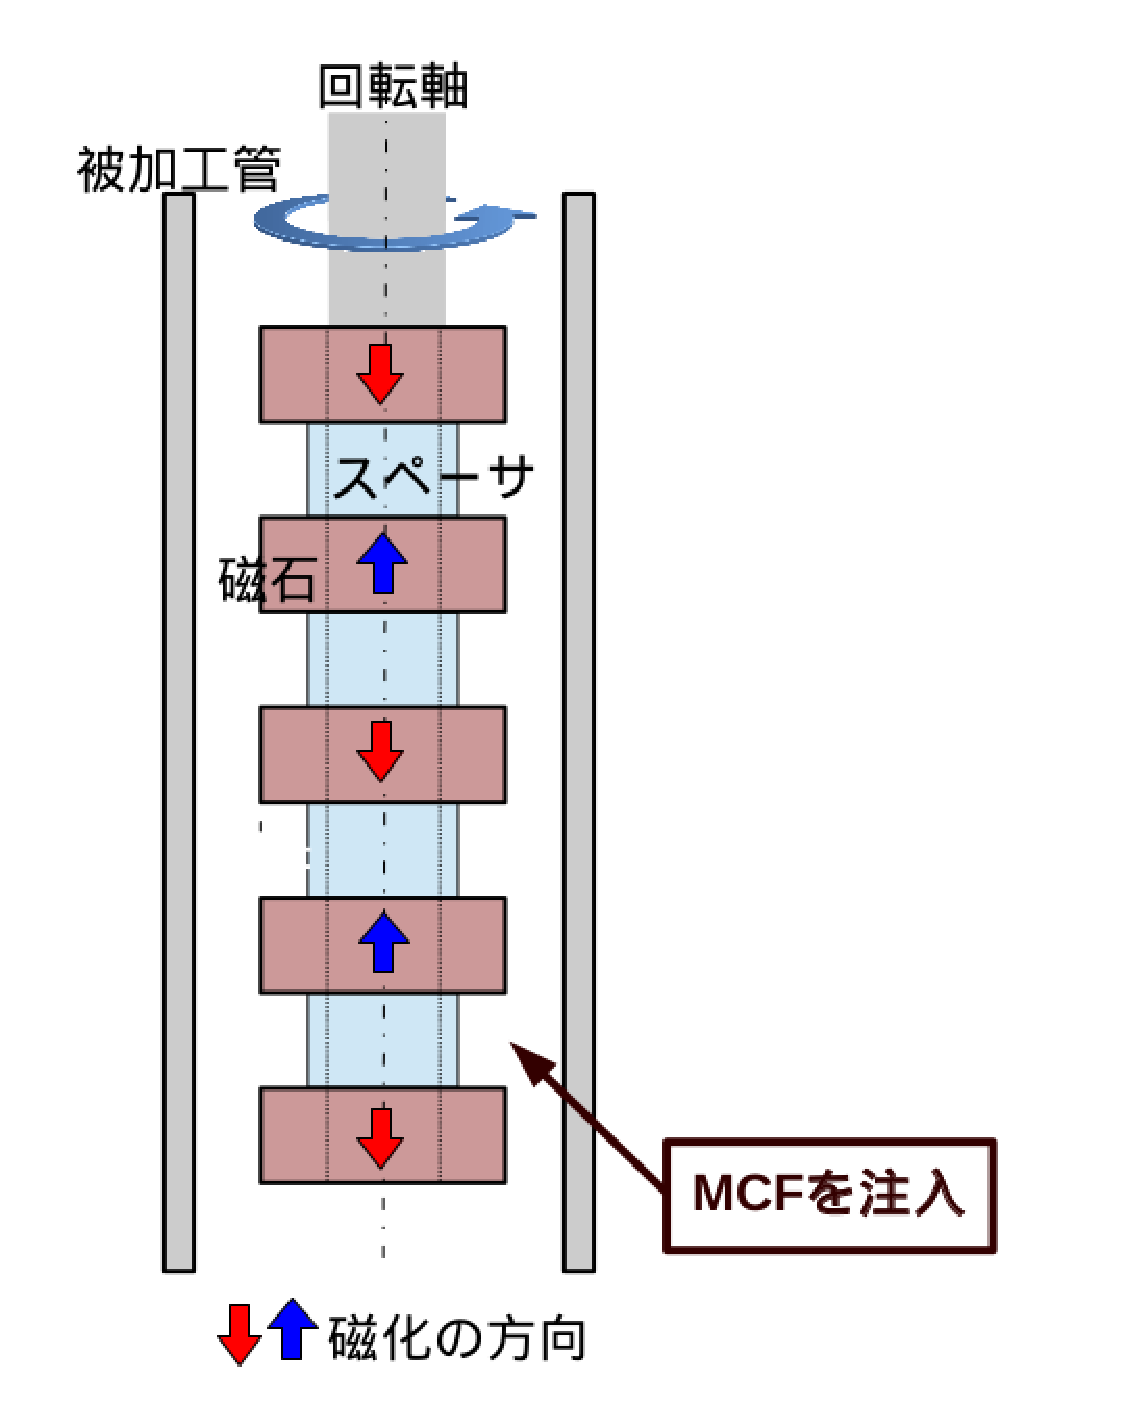
\includegraphics[height=90mm]{sd.eps}
      \end{center}
      \caption{研磨の様子の断面図}
      \label{fig:sd}
    \end{minipage}
    \begin{minipage}{0.5\hsize}
      \begin{center}
        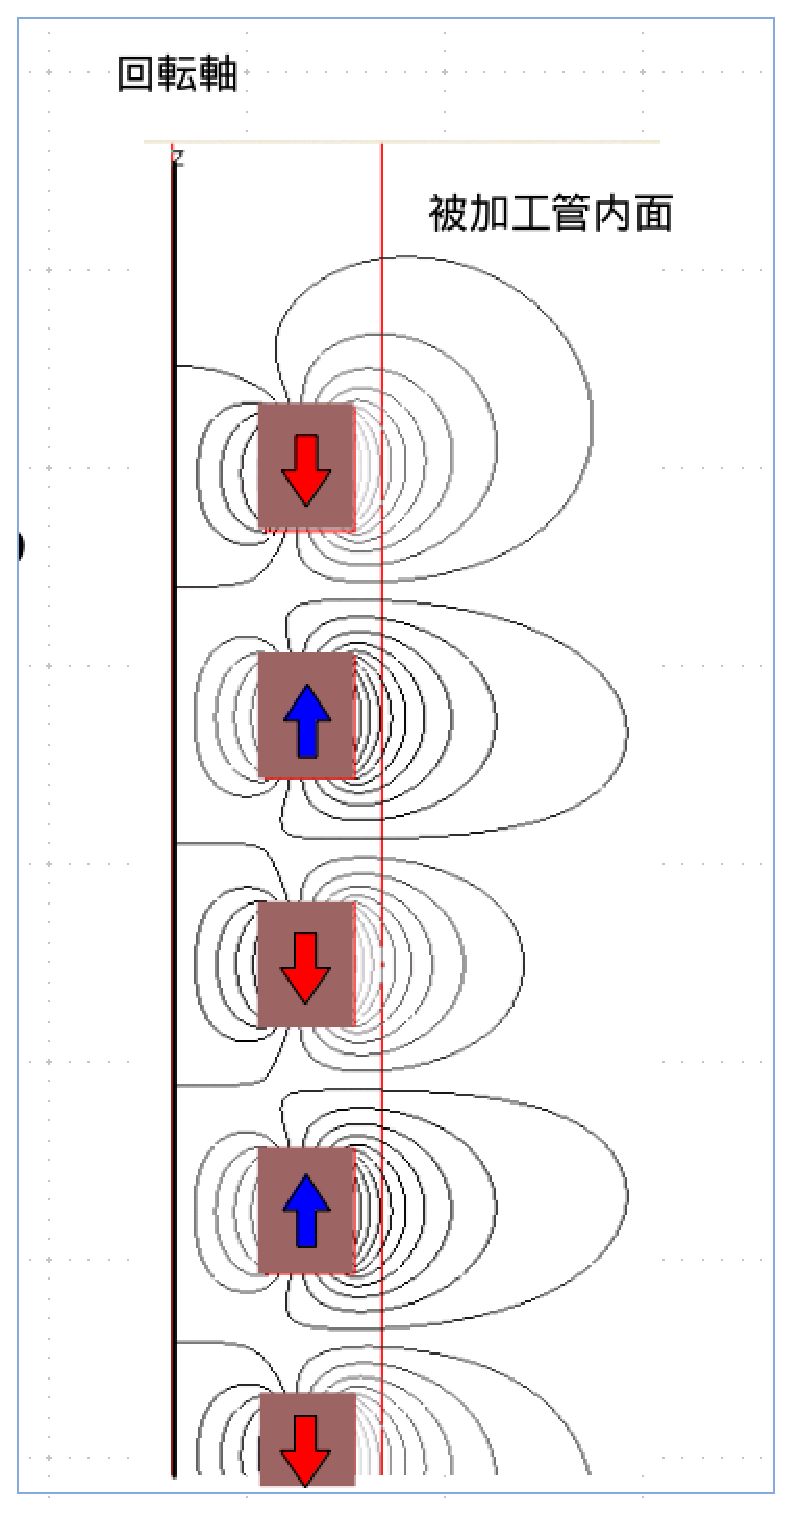
\includegraphics[height=90mm]{MagneticFlux.eps}
      \end{center}
      \caption{磁束分布の解析例}
      \label{fig:MagneticFlux}
    \end{minipage}
  \end{figure}

  \subsection{有限要素法にもとづく反復計算と変分法}
有限要素法とは微分方程式を数値的に解く際によく用いられ, 無限自由度の場を微小な有限の領域で区切り計算を行う. これによって微分方程式を節点同士の差分方程式に置き換え, それを解くことにより近似的に数値計算を行うことができる. 本研究では回転対称な静磁場についてマクスウェル方程式を解く際に2次元の有限要素法を適用した. 本解析では特にエネルギー密度が高い領域を重点的に分割するアダプティブオートメッシュを使用し, 動的に要素の分割数を増やしながら計算を行っている. この反復法の過程で近似の精度を高めてゆき, ある収束条件を満たすまでくり返し計算を行った. この定式化は物理的に変分法に対応する. 
\newpage

\section{被加工管内面での磁束密度の大きさ}
表\ref{tab:tool_size}に本研究で用いた工具寸法の一覧を示し, 図\ref{fig:TypeA_sd}, 図\ref{fig:TypeB_sd}, 図\ref{fig:TypeC_sd}, 図\ref{fig:Typealpha_sd}, 図\ref{fig:Typebeta_sd}に工具の模式図を示した. 特に図\ref{fig:Typealpha_sd}に工具構成要素の凡例を示し, 図\ref{fig:Typebeta_sd}に磁束密度成分の凡例を示した. 工具TypeA, TypeB, TypeCを比較すると, 磁石の寸法はすべて同じだがスペーサの寸法についてTypeAでは外径がTypeBやTypeCと異なり, 磁性流体の充填量が異なる. またTypeBとTypeCでスペーサの外径は等しいが, 厚みが異なる. 工具Type$\alpha$とType$\beta$では外径は同じだが磁石幅とスペーサの幅がそれぞれ異なり, TypeA, TypeB, TypeCには無かった工具カバーがされている. 
被加工管内面での磁束密度の大きさについて, 2通りの工具形状の計測実験結果と磁界シミュレーションでの解析結果を比較し, 解析結果の妥当性を検証した. なおこの計測実験は西田ら\cite{西田}によるものである. 図\ref{fig:TypeAB_B}にTypeA, TypeBの被加工管内面での軸方向の磁束密度の分布を, 図\ref{fig:TypeC_B}にTypeCでの磁束密度の分布を示す. 磁束密度の分布図で青色のハッチングで示した領域は磁石がある領域に対応し, 模式図で赤色で示した線分は実測実験が行われ分布をプロットした領域である. また図\ref{fig:TypeA_sd}, 図\ref{fig:TypeB_sd}に工具TypeA, Bにおける工具の模式図を, 図\ref{fig:TypeC_sd}に工具TypeCにおける工具の模式図を示し, 解析の際に設定した磁石の物理特性と計測に用いた永久磁石の物理特性を表\ref{tab:magnet_property}にそれぞれ示す. 表\ref{tab:magnet_property}中でMaterial N-40は磁石の製造もとである二六製作所が公開したものである. NdFe30とNdFe35はMaxwell SVの内部データベースの中から類似の材質を引用したものである. この2種類の材質を用いてシミュレーションを行った. \par
おおむね工具TypeA, TypeB, TypeCともによい対応がとれており, 磁石のなかほどと磁石と磁石の間では特によい対応がある. 最大相対誤差は12\%程度であった. しかし磁石の端面周辺に対応する領域で解析値と測定値ともに磁束密度の大きさが最大値をとっているが, その軸方向位置には0.5mm程度のずれが確認できる. またTypeA,Bはスペーサの寸法のみが異なるが, スペーサは非磁性体であるため測定された磁束密度の分布にその影響は現れていない. \par
実測値については着磁方向の分散, 残留磁束密度のばらつきの影響をうけ, 測定位置が磁極に近く位置ずれによる磁束密度変化は大きく現れる. さらにガウスメータのプローブがもつ大きさと形状による影響や磁石の面取りの影響も受ける. それでも解析結果との誤差は最大となる位置でも12\%程度であった. 定性的にも磁界強度分布の傾向は一致しており, 実験結果を評価する上で十分な確度の解析結果であると判断した. 

  \begin{table}[H]
    \begin{tabular}{|c||c|c|c|} \hline
        Tool Type & Number of Magnet & Size of Magnet [mm] & Size of Spacer [mm] \\ \hline \hline
        TypeA & 5 & φ13 × φ6 × 5 & φ13 × 2.5  \\ \hline
        TypeB & 5 & φ13 × φ6 × 5 & φ8 × 2.5   \\ \hline
        TypeC & 5 & φ13 × φ6 × 5 & φ8 × 5   \\ \hline
        Type$\alpha$ & 5 & φ12 × φ6 × 5 & φ12 × 2.5   \\ \hline
        Type$\beta$ & 5 & φ12 × φ6 × 3 & φ12 × 1.5   \\ \hline
    \end{tabular}
    \centering
    \caption{工具寸法}
    \label{tab:tool_size}
  \end{table}

  \begin{figure}[H]
    \begin{center}
      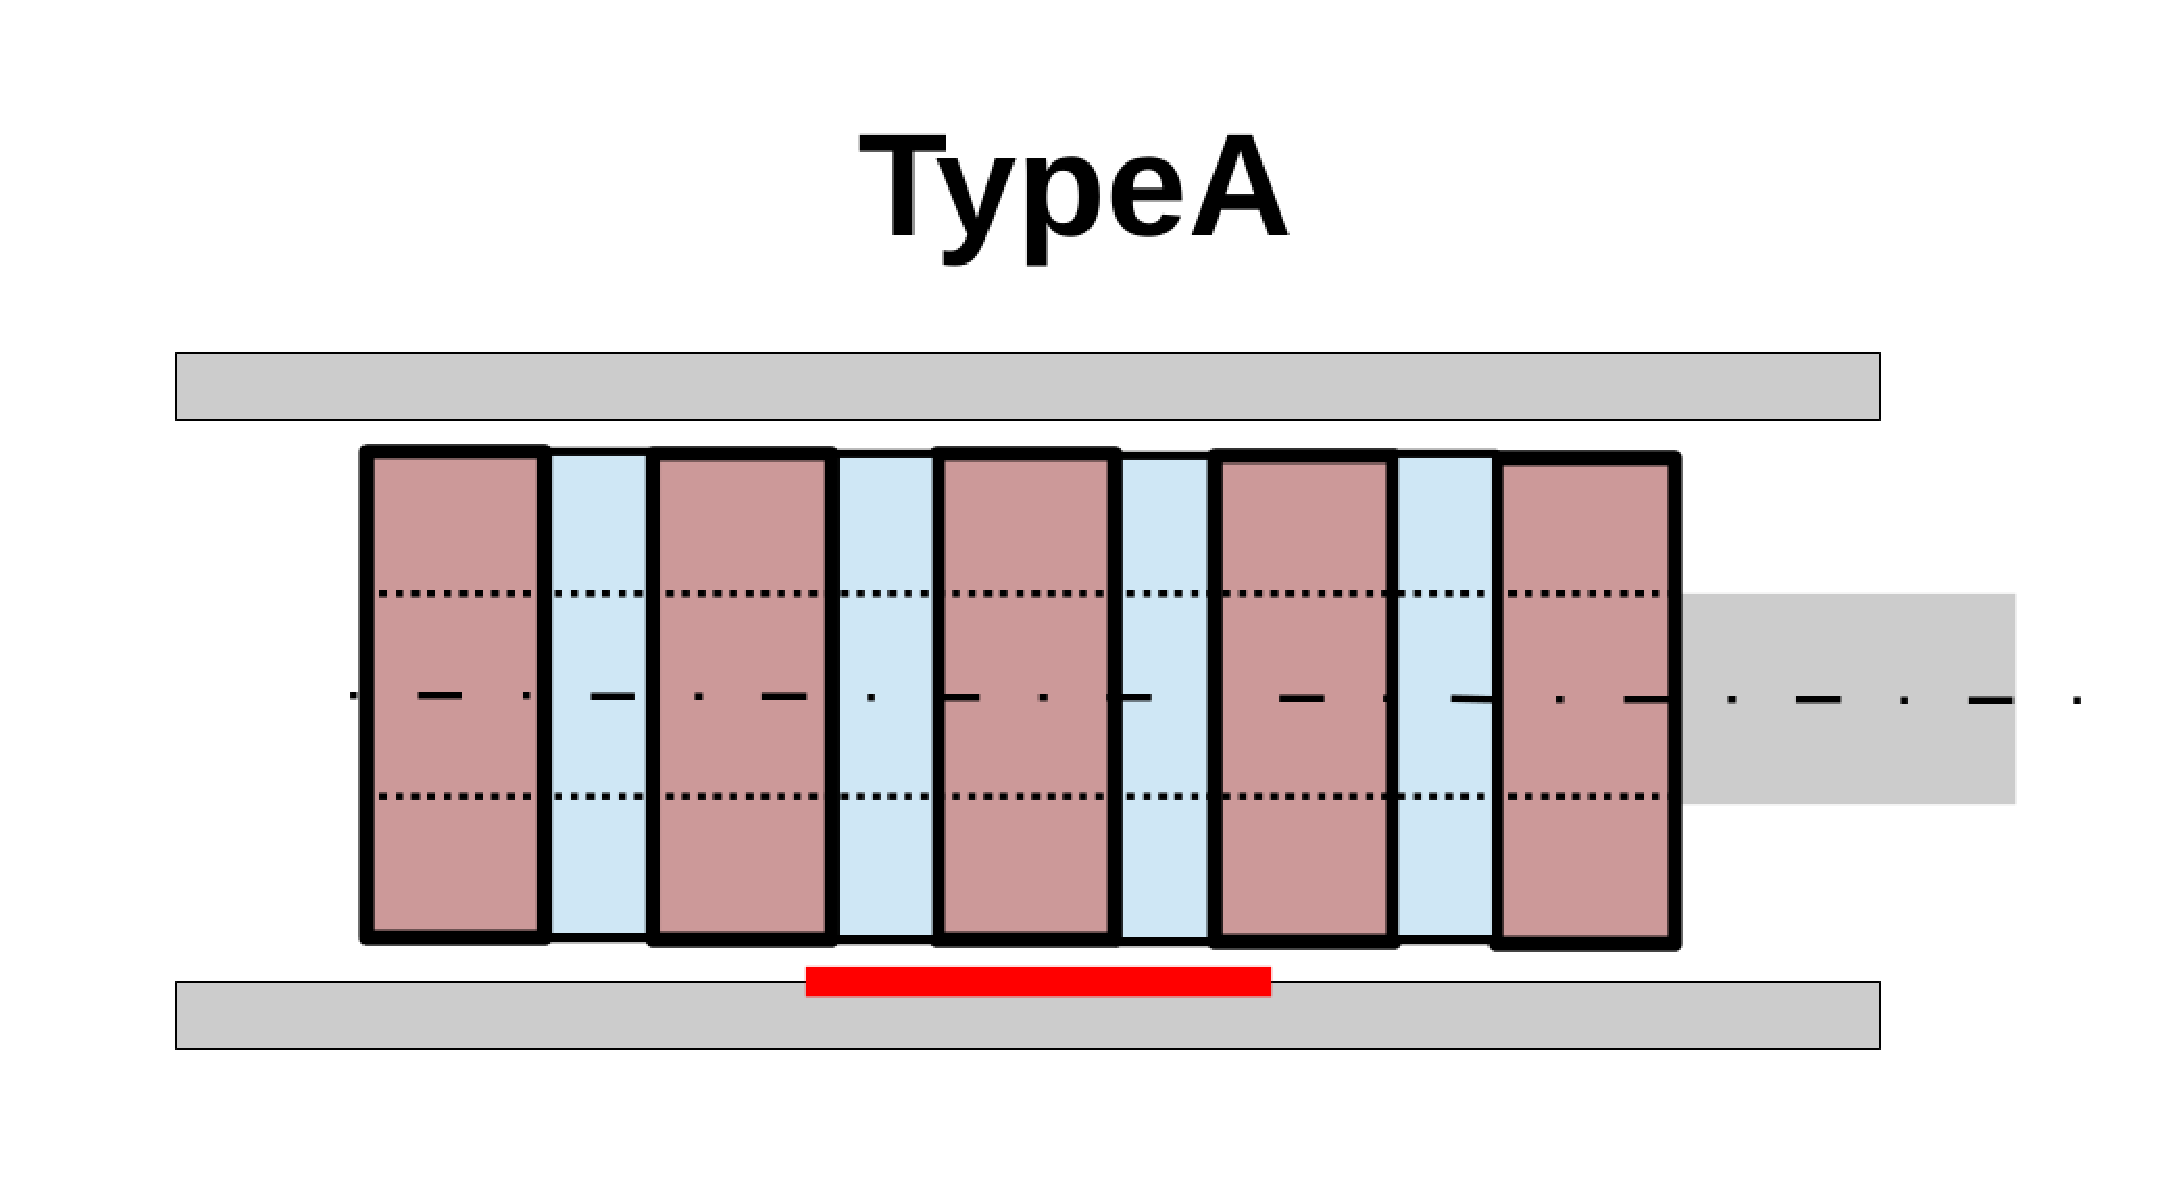
\includegraphics[width=75mm]{TypeA_sd.eps}
    \end{center}
    \caption{工具模式図(TypeA)}
    \label{fig:TypeA_sd}
  \end{figure}

  \begin{figure}[H]
    \begin{center}
      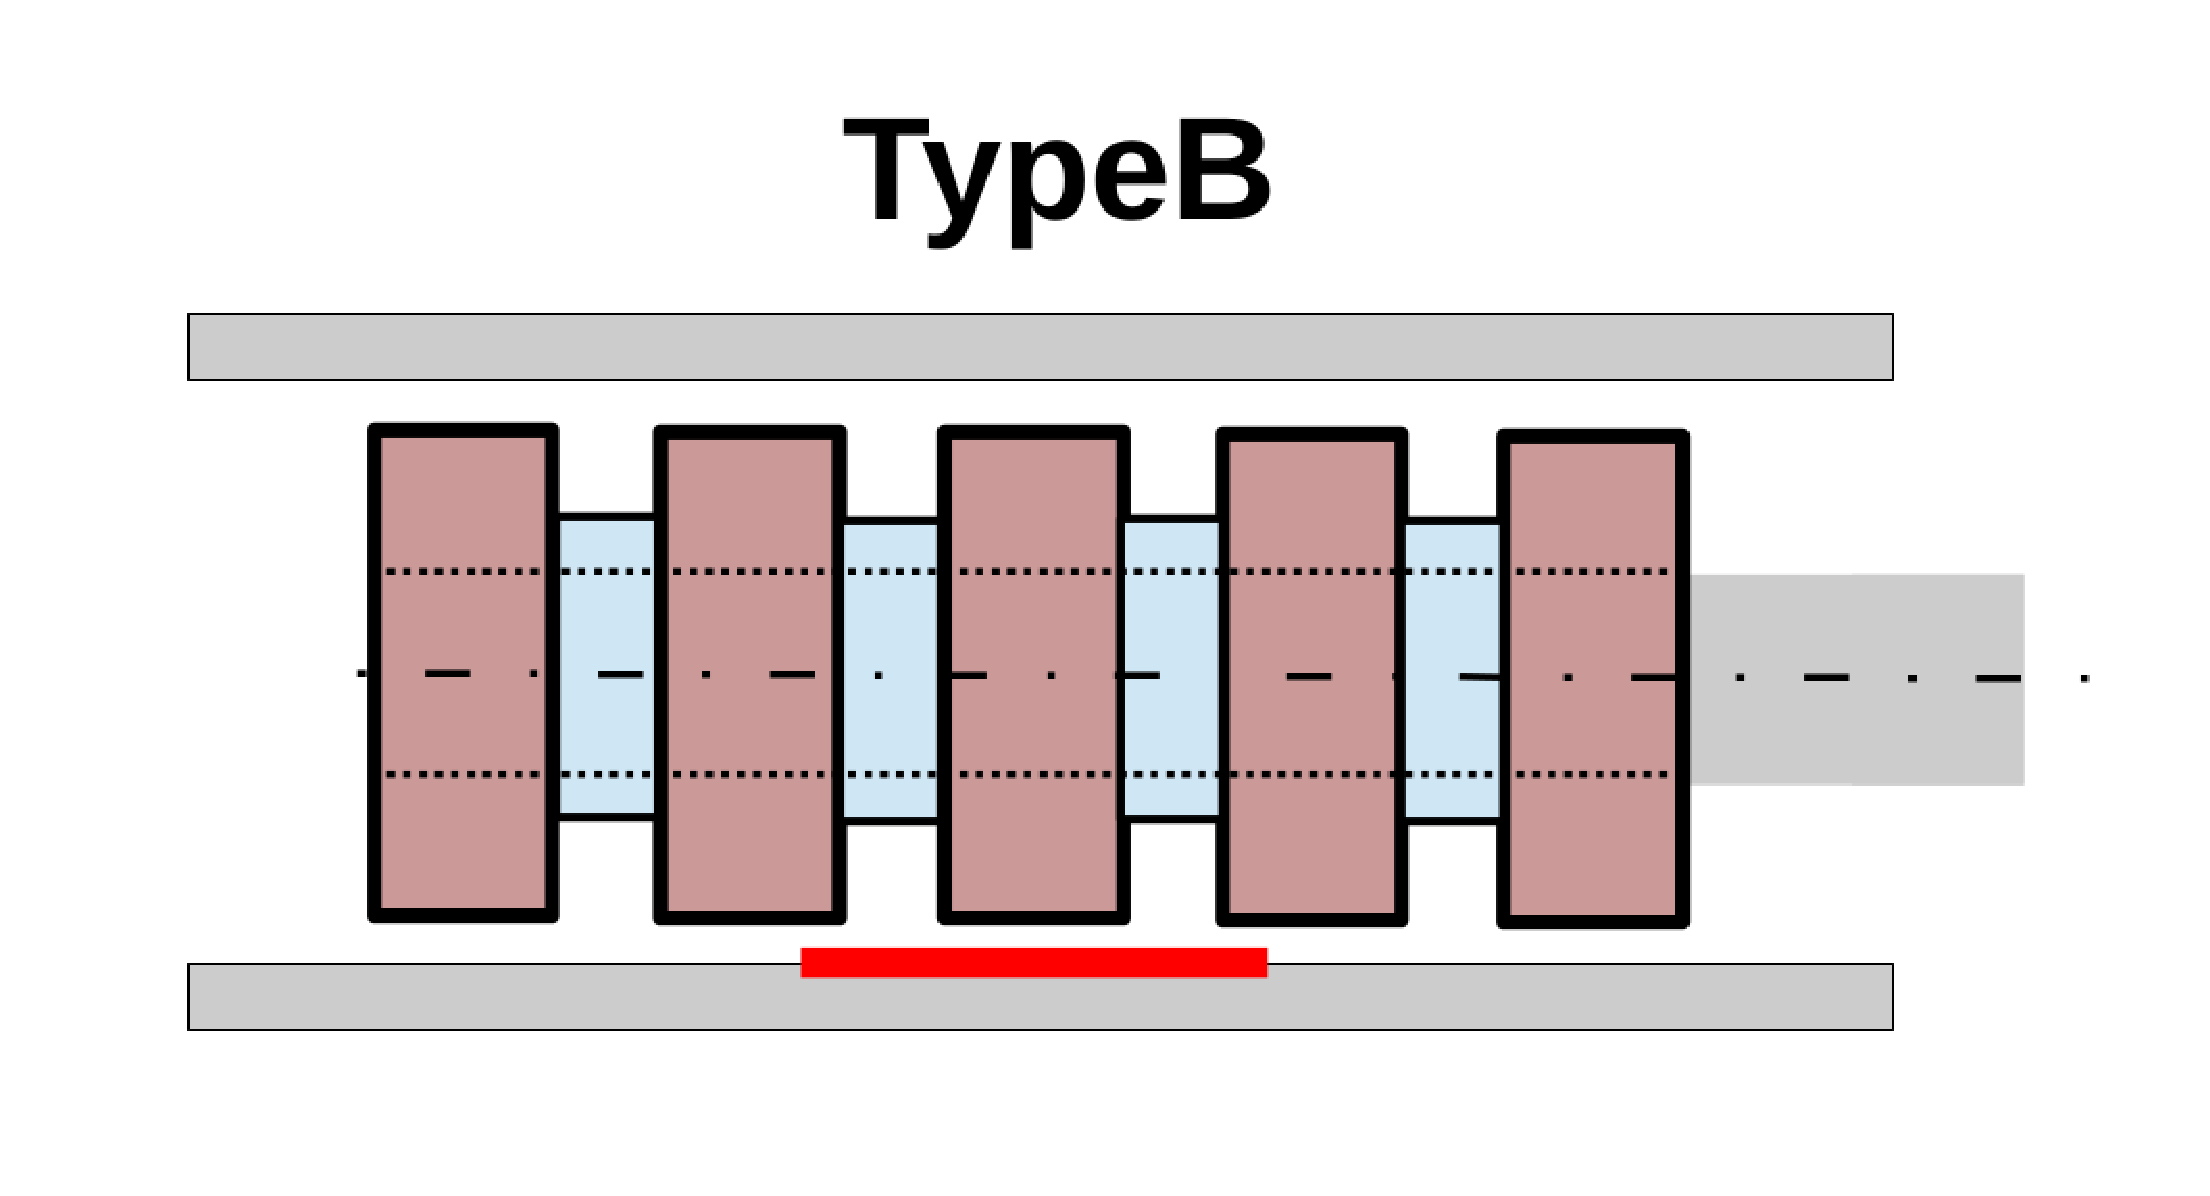
\includegraphics[width=75mm]{TypeB_sd.eps}
    \end{center}
    \caption{工具模式図(TypeB)}
    \label{fig:TypeB_sd}
  \end{figure}

  \begin{figure}[H]
    \begin{center}
      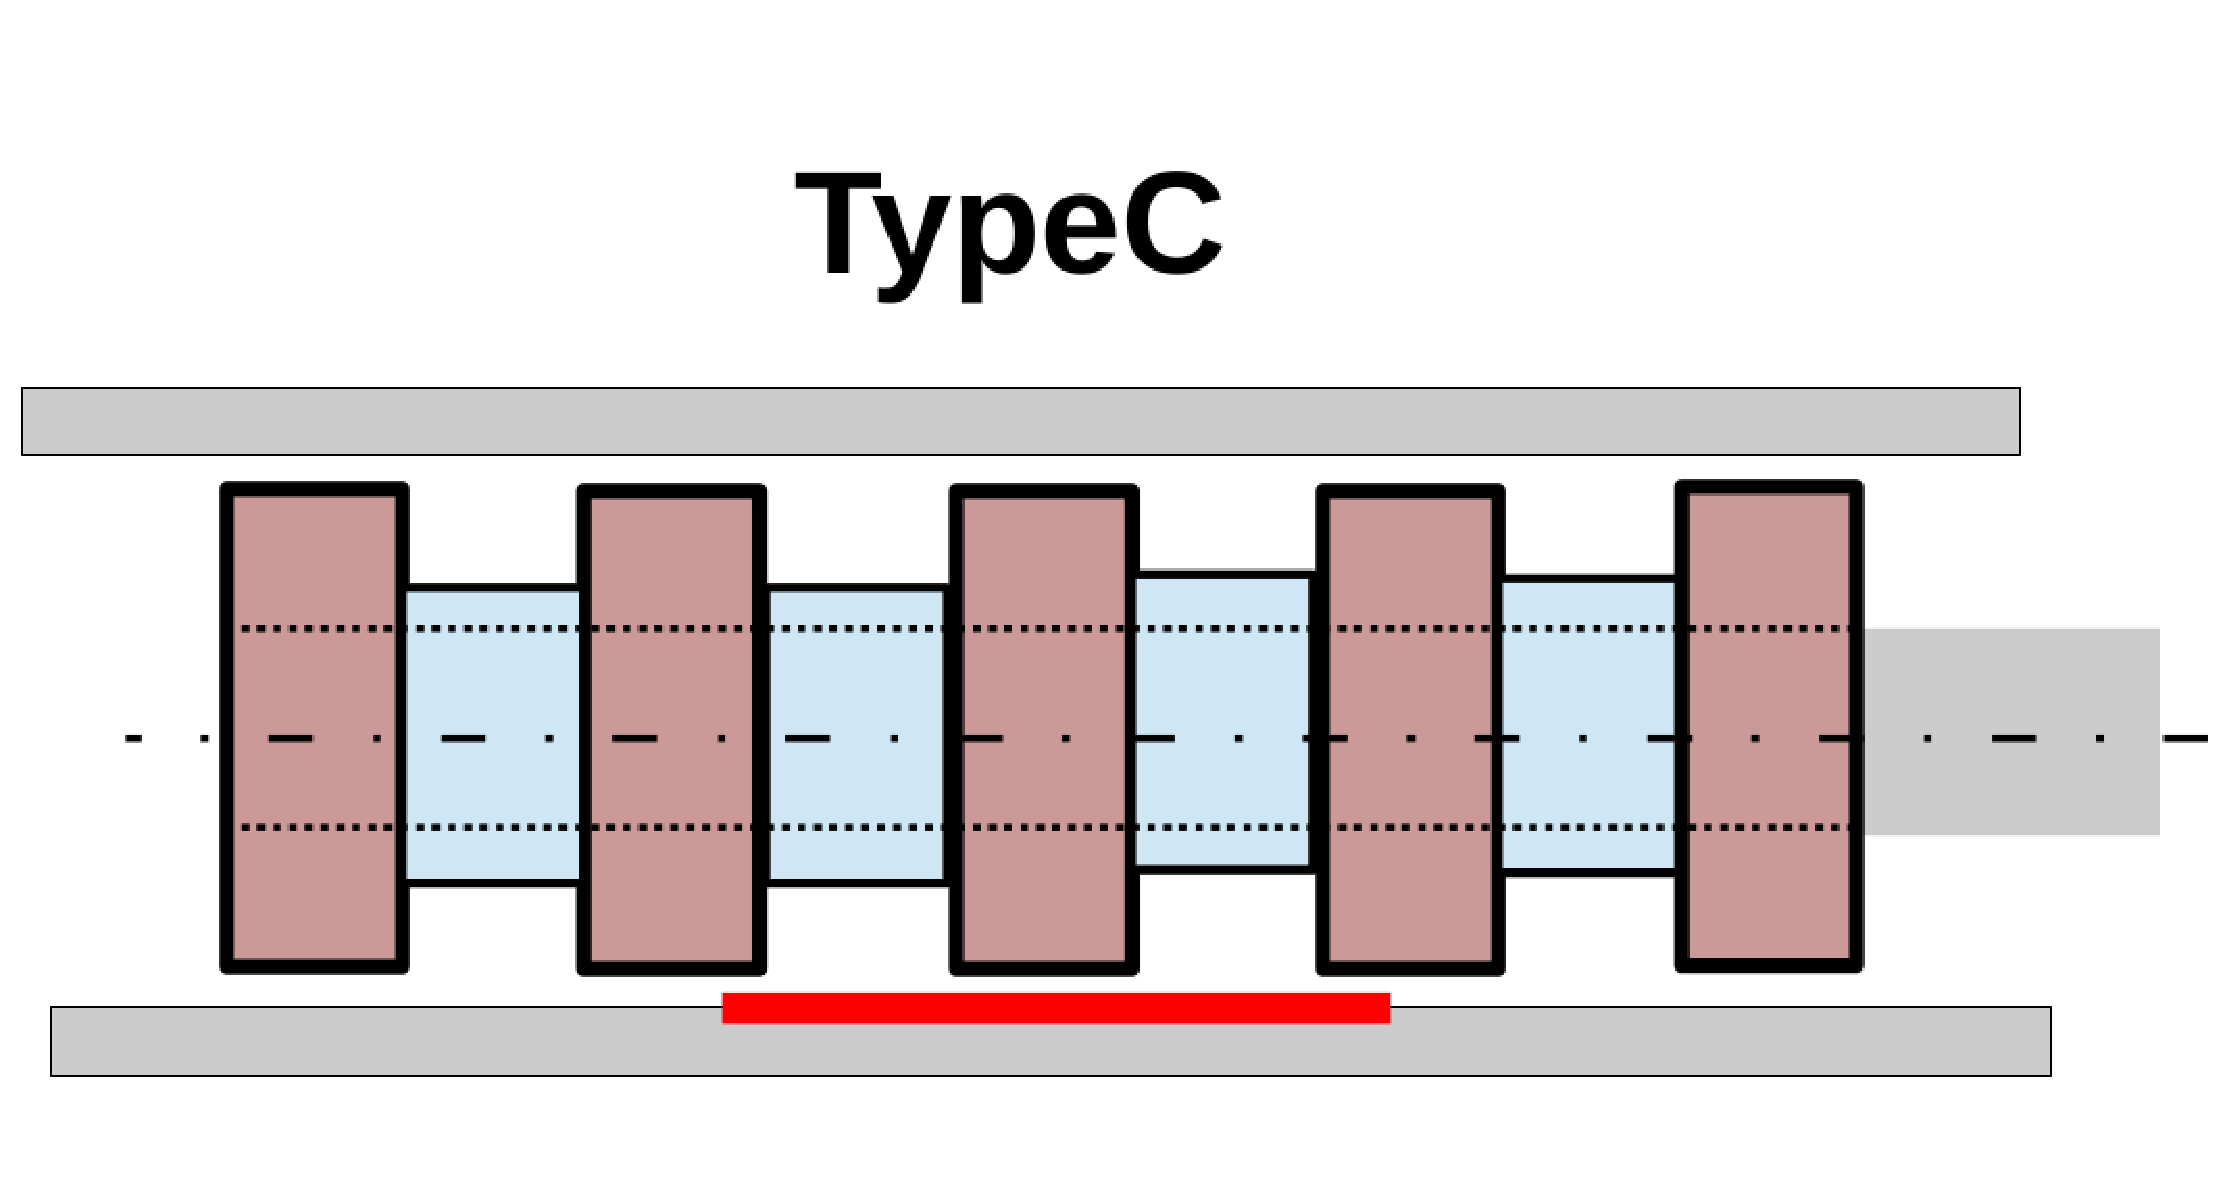
\includegraphics[width=75mm]{TypeC_sd.eps}
    \end{center}
    \caption{工具模式図(TypeC)}
    \label{fig:TypeC_sd}
  \end{figure}

  \begin{figure}[H]
    \begin{center}
      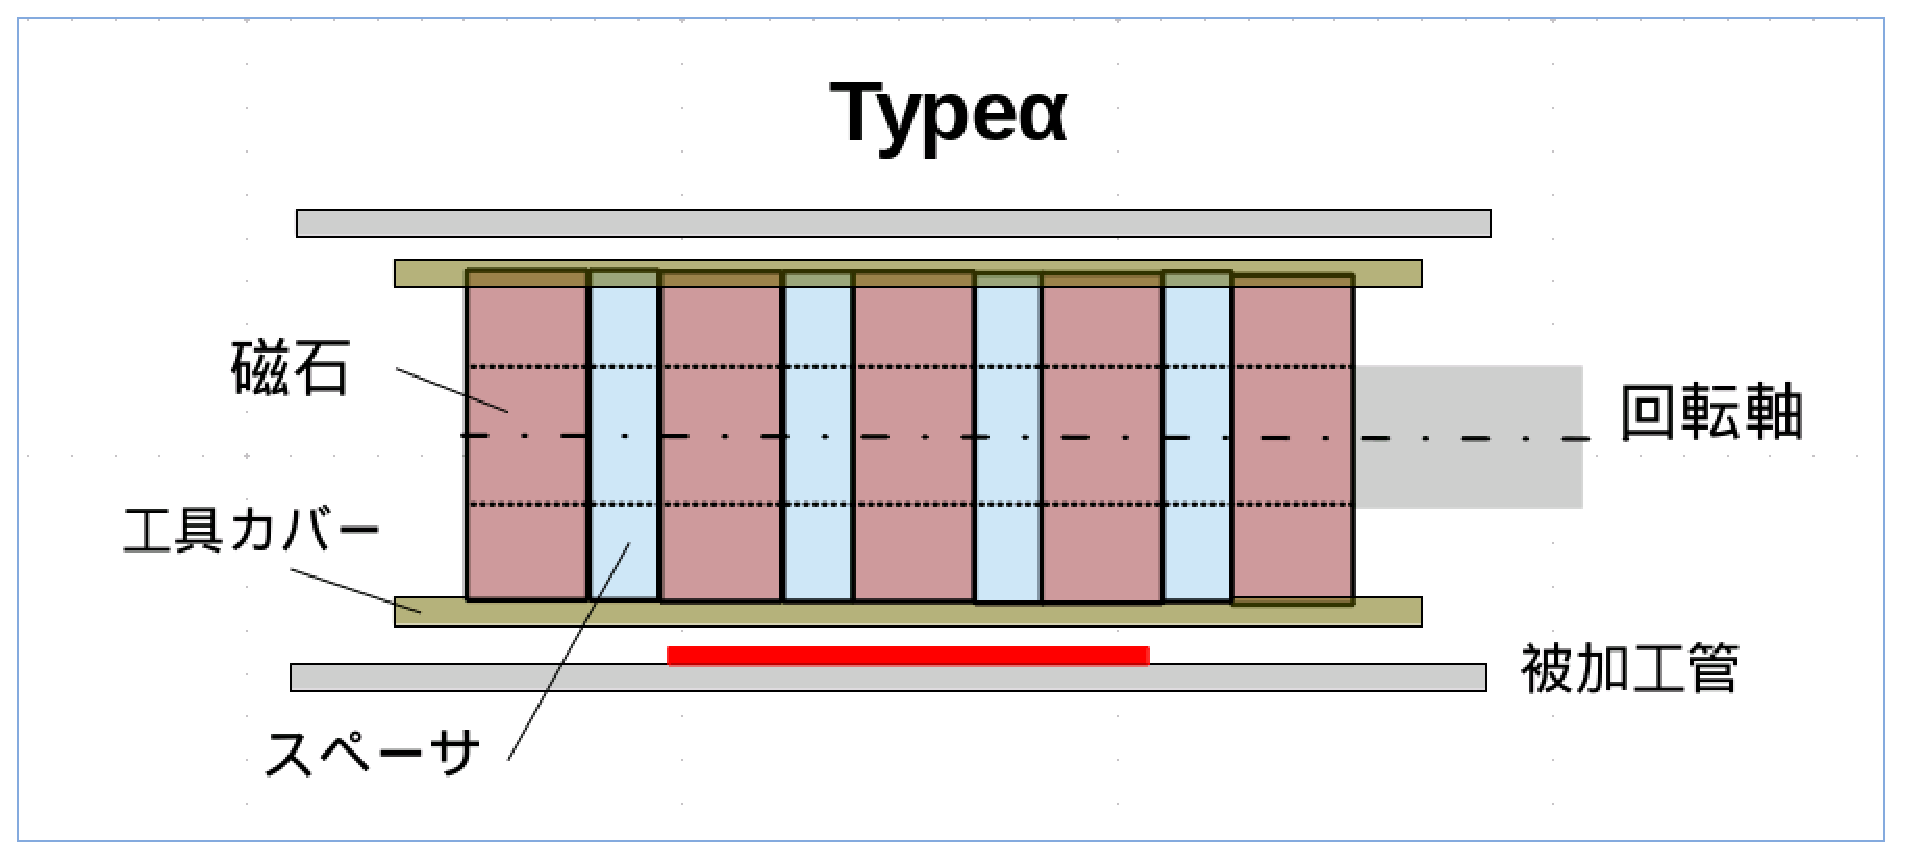
\includegraphics[width=110mm]{Typealpha_sd.eps}
    \end{center}
    \caption{工具模式図(Type$\alpha$)}
    \label{fig:Typealpha_sd}
  \end{figure}

  \begin{figure}[H]
    \begin{center}
      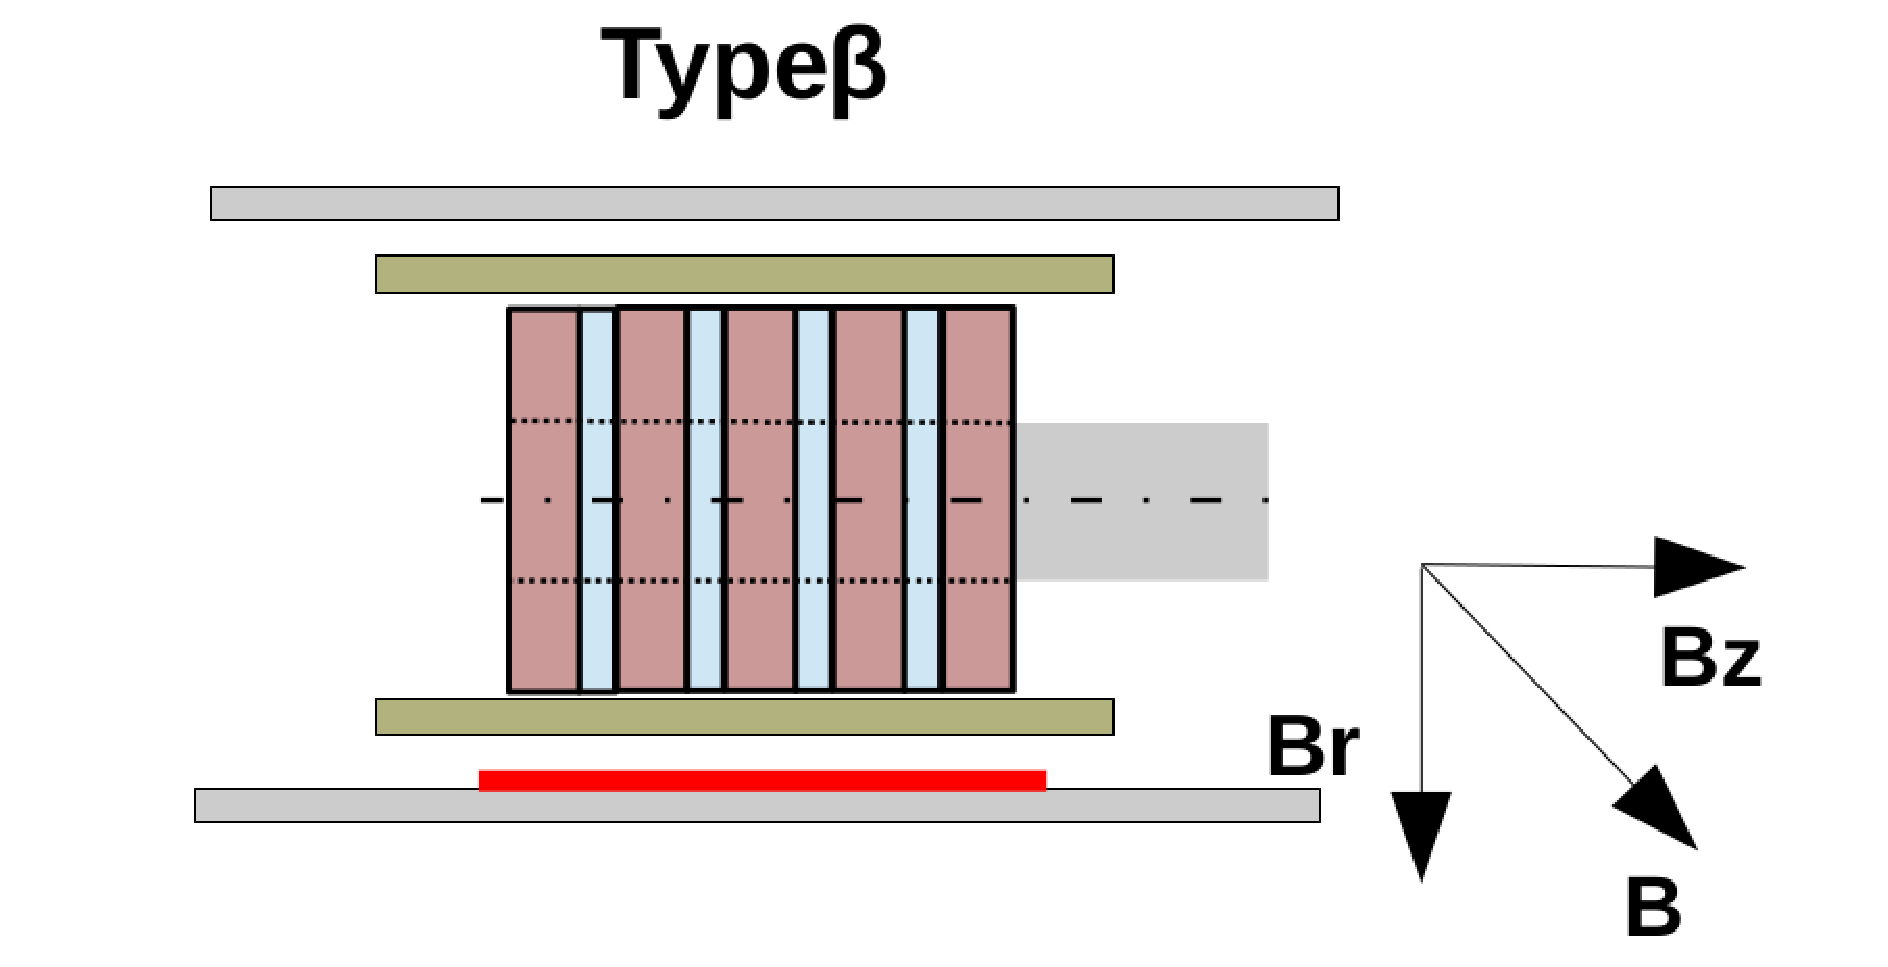
\includegraphics[width=90mm]{Typebeta_sd.eps}
    \end{center}
    \caption{工具模式図(Type$\beta$)}
    \label{fig:Typebeta_sd}
  \end{figure}

  \begin{figure}[H]
    \begin{center}
      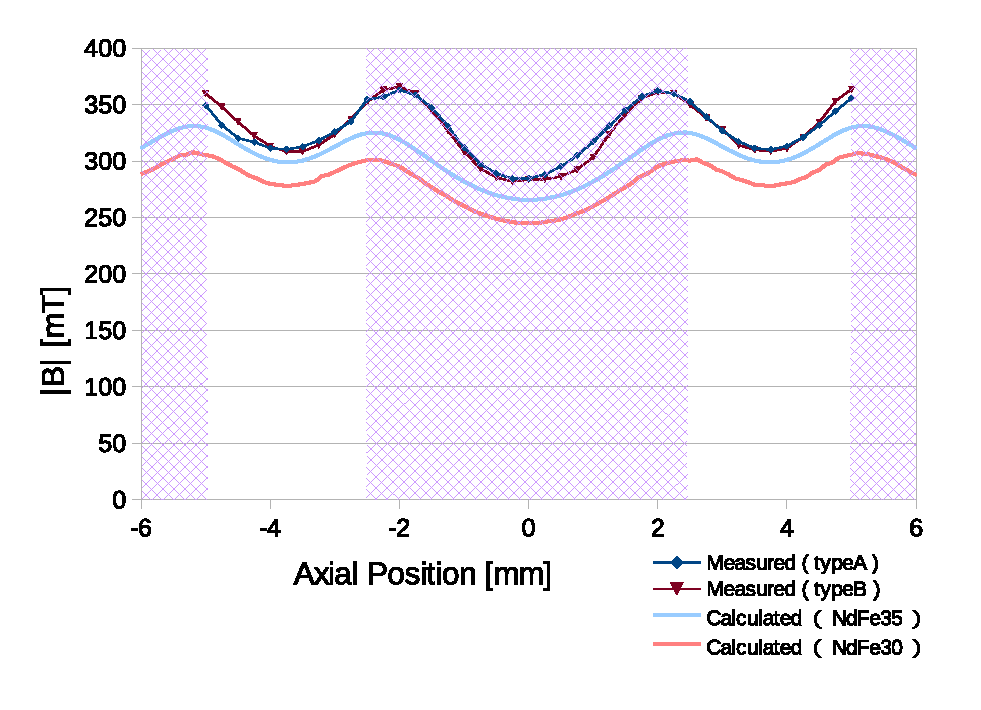
\includegraphics[width=130mm]{TypeAB_B.eps}
    \end{center}
    \caption{被加工管内面における磁束密度の大きさの分布(TypeA,B)}
    \label{fig:TypeAB_B}
  \end{figure}

  \begin{figure}[H]
    \begin{center}
      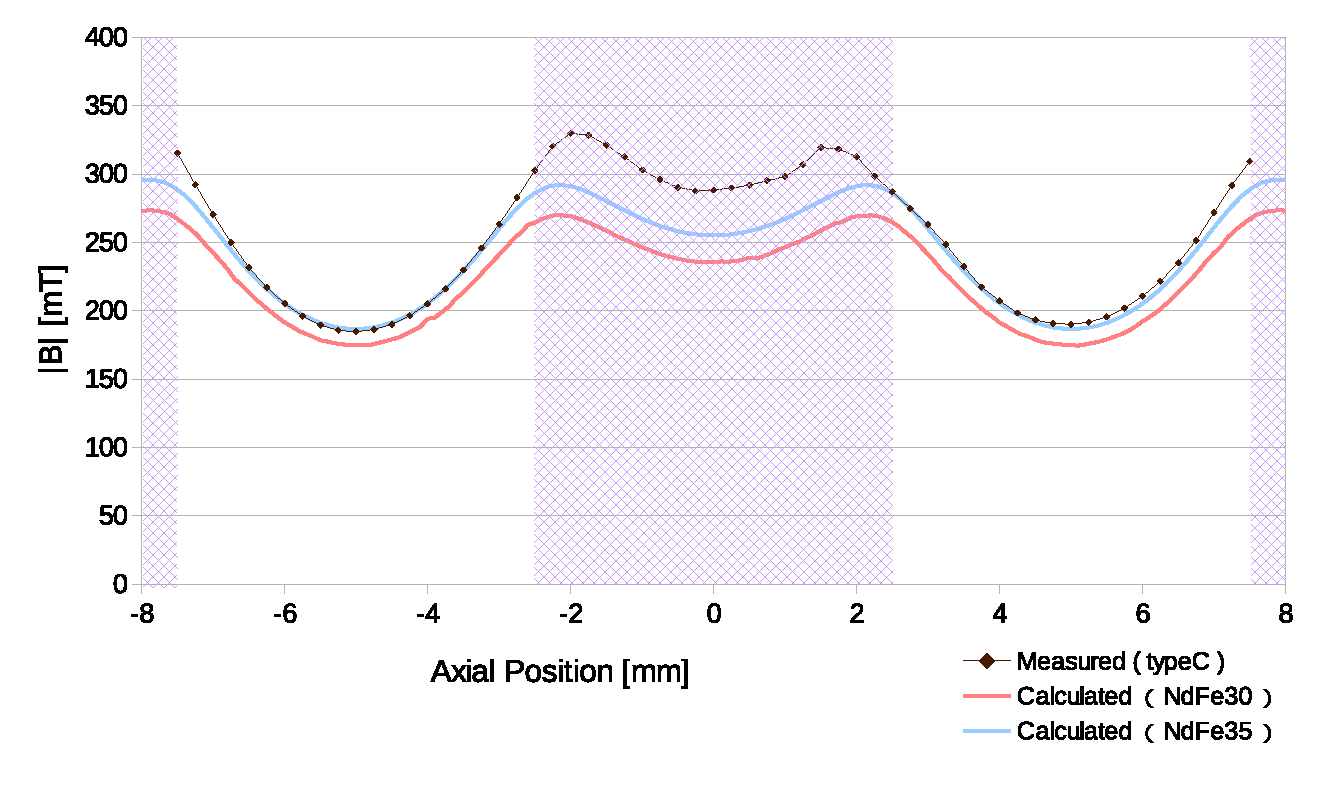
\includegraphics[width=150mm]{TypeC_B.eps}
    \end{center}
    \caption{被加工管内面における磁束密度の大きさの分布(TypeC)}
    \label{fig:TypeC_B}
  \end{figure}

  \begin{table}[H]
    \begin{tabular}{||l||c|c||} \hline \hline

      & Relative Permeability $\mu_r$ & Magnetic Retensivity $B_r$[T] \\ \hline
      Material N-40* & - & 1.25 $\sim$ 1.32  \\ \hline
      Model: NdFe30 & 1.045 & 1.10 \\ \hline
      Model: NdFe35 & 1.099 & 1.23 \\ \hline \hline

     & Magnetic Coercivity {\it bHc}[A/m] & Magnetic Coercivity {\it iHc}[A/m] \\ \hline
      Material N-40* & $\geq$859000 & $\geq$955000 \\ \hline
      Model: NdFe30 & 828000 & - \\ \hline
      Model: NdFe35 & 890000 & - \\ \hline \hline

     & \multicolumn{2}{|c|}{ Maximum Energy Product $BH_{max}{\rm [J/m^3]}$ } \\ \hline
      Material N-40* & \multicolumn{2}{|c|}{ 302000 $\sim$ 334000 } \\ \hline
      Model: NdFe30 & \multicolumn{2}{|c|}{ - } \\ \hline
      Model: NdFe35 & \multicolumn{2}{|c|}{ - } \\ \hline \hline

    \end{tabular}
    \centering
    \caption{磁石の磁気特性}
    \label{tab:magnet_property}
  \end{table}

\begin{comment}
  \subsection{変分定理にもとづいた解析結果の検討}
 有限要素法を用いた解析の特性上, 解析結果を出力する際に分割された領域の内部ではその境界での情報を用いて, 物理量の補完が行われている. また反復法を用いた計算の過程で領域を動的に分割してゆく場合, 反復回数を増やし領域の分割数を増やすと領域内部での近似の精度は単調に高くなり, 物理量はより滑らかに補完される. \\
 本研究では図\ref{fig:TypeAB_B}, 図\ref{fig:TypeC_B}から, 被加工管内面での磁束密度の大きさは概ね滑らかに接続されていると考えることができるが, 一部なめらかでない領域が存在する. 反復回数を大きくして領域の分割数を増やすとより滑らかになることが確認されているが, 本研究では定性的な考察が特に重要であり, また網羅的にさまざまな寸法について解析をおこなうため, 計算時間とトレードオフの関係にある解析精度の高さを高めることができなかった. \\
 なお本解析では反復法における収束判定条件としてステップ毎の評価関数$f_{eval}$の偏差$\epsilon$を用いており, ステップ毎の相対偏差$\epsilon$があるし
きい値$\epsilon_{lim}$(ただし$\forall \epsilon_{lim} \le 0.0003$)を下回ったとき十分に精度良く評価関数$f_{eval}$が収束しているとし計算を終了した. 収束の評価関数としては, 変分定理にもとづき系のエネルギーもしくはエネルギー密度をもちいている. \\
\end{comment}

\newpage

\section{解析結果と加工実験結果との比較}
加工原理への考察を行うため, 2種類の工具において加工量と磁場解析結果をそれぞれ比較した. 加工実験は楠ら\cite{楠}によるもので20分間, 工具の回転数は750rpm, 1000rpm, 1250rpm, 1500rpmのそれぞれにおいて加工をおこなっている. また工具Type$\alpha$についての解析結果を用いてMCFに含まれる鉄粉に働く様々な力を概算し評価した. 

  \subsection{磁束密度と加工量との比較}
図\ref{fig:Typealpha_B}に工具Type$\alpha$での磁束密度の大きさの径方向成分Br, 軸方向成分Bz, その大きさBと加工量を比較したグラフを示した. なお工具Type$\alpha$について模式図を図\ref{fig:Typealpha_sd}に示し, その寸法を表\ref{tab:tool_size}に示す. 図\ref{fig:deltaR_sd}に模式的に示したように, 内径変化量は加工量に対して符号が反転したものに対応する. すなわち内径変化量が負に小さければ小さいほど, 加工量は大きいことを意味する. \par
図\ref{fig:Typealpha_B}からわかるように被加工管内面での磁束密度の大きさが磁石のなかほどで小さくなっているのに対し, 加工量は大きくなっている. また逆に磁束密度の大きさが大きくなっている磁石の間で加工量は小さくなっている. 表\ref{tab:CC_alpha}に磁束密度の径方向成分と軸方向成分, 磁束密度の大きさと加工量の組み合わせについて, 工具回転数750rpm, 1000rpm, 1250rpm, 1500rpmそれぞれ相関係数を求めたものを示した. なお後で鉄粉に働く様々な力を概算する際には, 磁場の強さを$1.6\times10^5$[A/m]程度とした. \par
磁束密度の大きさに関して, すべての回転数について加工量と負の相関があることがわかる. すなわち磁束密度の大きさと加工量の間に直接的な関連性をみいだすことはできないことが分かった. また磁束密度の軸方向成分に関しては加工量と正の相関があることがわかる. \par
同様に図\ref{fig:Typebeta_B}に工具Type$\beta$での磁束密度の分布と加工量, 図\ref{fig:Typebeta_sd}に模式図を示し, 寸法を表\ref{tab:tool_size}に示す. また表\ref{tab:CC_alpha}に相関係数を示した. 工具Type$\beta$でも磁束密度の大きさと加工量の間に直接的な関連性をみいだすことはできない. 

 \subsection{磁束密度の勾配と加工量との比較}
図\ref{fig:Typealpha_B}, 図\ref{fig:Typebeta_B}に工具Type$\alpha$, Type$\beta$それぞれでの磁束密度の大きさの径方向への微分係数と加工量について比較したグラフを示した. 磁束密度の大きさの径方向への微分係数は磁束密度の勾配に対応しており, 式\ref{eq:prop}に示したように磁束密度の勾配は磁気浮揚力と近似的に比例関係にあることが知られている\cite{磁性流体}. なお後で鉄粉に働く様々な力を概算する際には,磁場の強さの径方向への偏微分係数を$1.1\times10^8[A/m^2]$程度とした. \par
図\ref{fig:Typealpha_B}, 図\ref{fig:Typebeta_B}から分かるように, 磁石の端に対応する領域では磁束密度の勾配が大きくなっているのに対して加工量は小さい. また磁石のなかほどに対応する領域ではその逆に, 磁束密度の勾配が小さくなっているのに対して加工量は大きい. このことから磁束密度の勾配と加工量は対応がとれておらず, 磁気浮揚力は加工量と関連性があるととらえることが難しいことが分かった. 

  \begin{eqnarray}
    F_{mb} & = &  v \bm{M} \cdot \nabla \bm{H} \nonumber \\
               & \propto &  \nabla \bm{M} \label{eq:prop}
  \end{eqnarray}

  \begin{figure}[H]
    \begin{center}
      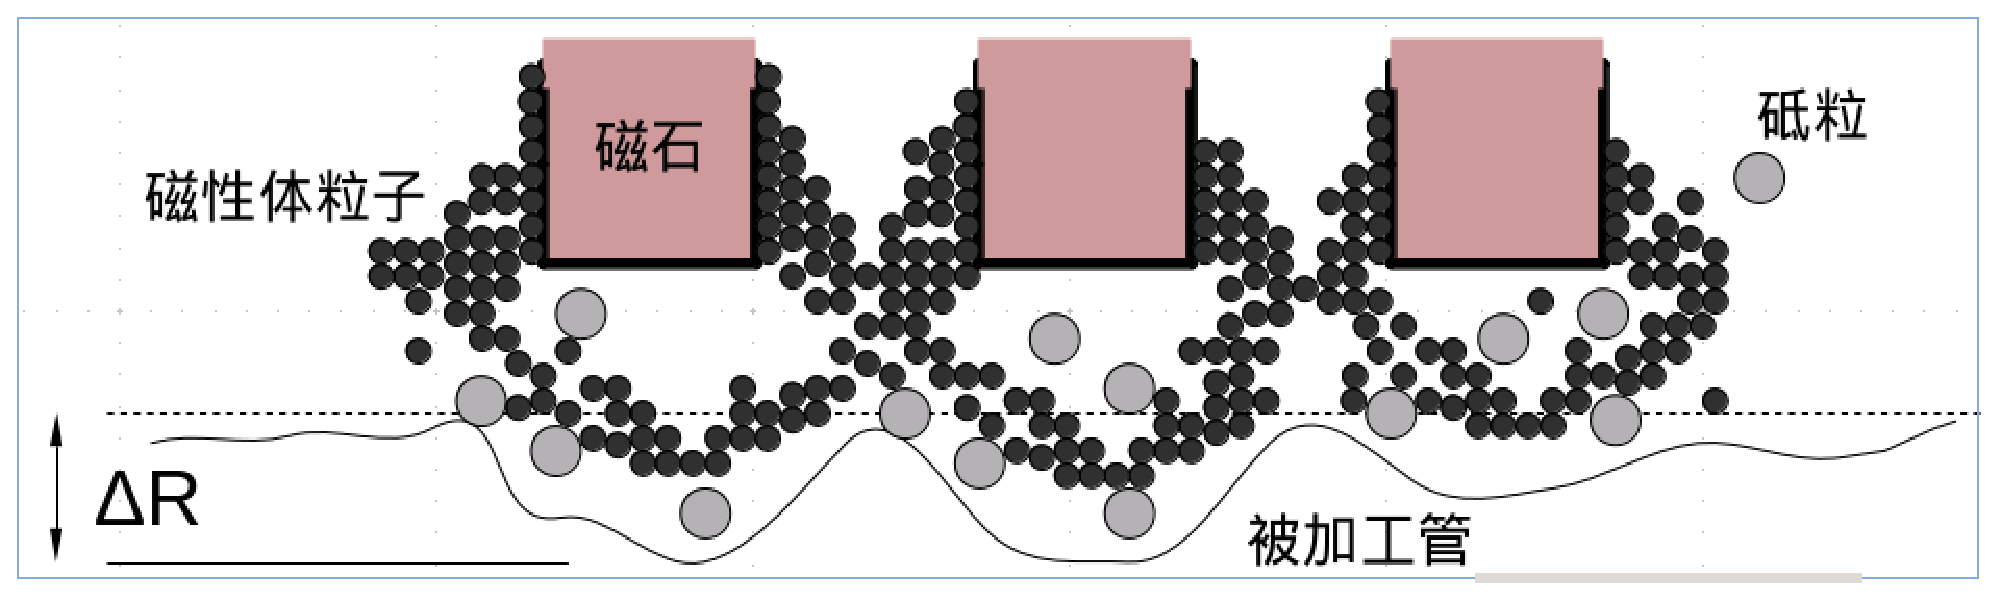
\includegraphics[width=100mm]{deltaR_sd.eps}
    \end{center}
    \caption{内径変化量模式図}
    \label{fig:deltaR_sd}
  \end{figure}

  \begin{figure}[H]
    \begin{center}
      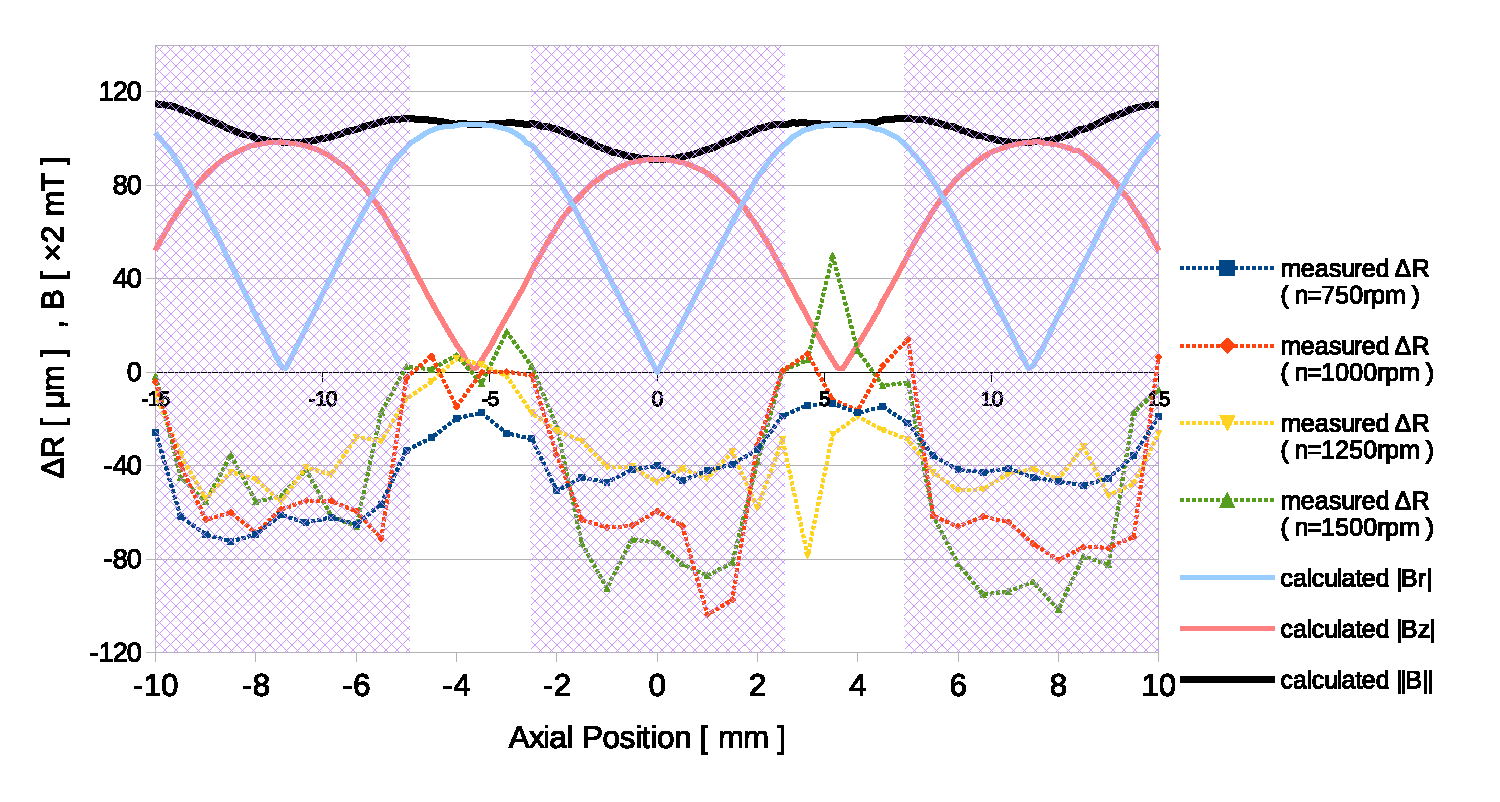
\includegraphics[width=150mm]{Typealpha_B.eps}
    \end{center}
    \caption{研磨加工による内径変化と磁束密度(Type$\alpha$)}
    \label{fig:Typealpha_B}
  \end{figure}

  \begin{figure}[H]
    \begin{center}
      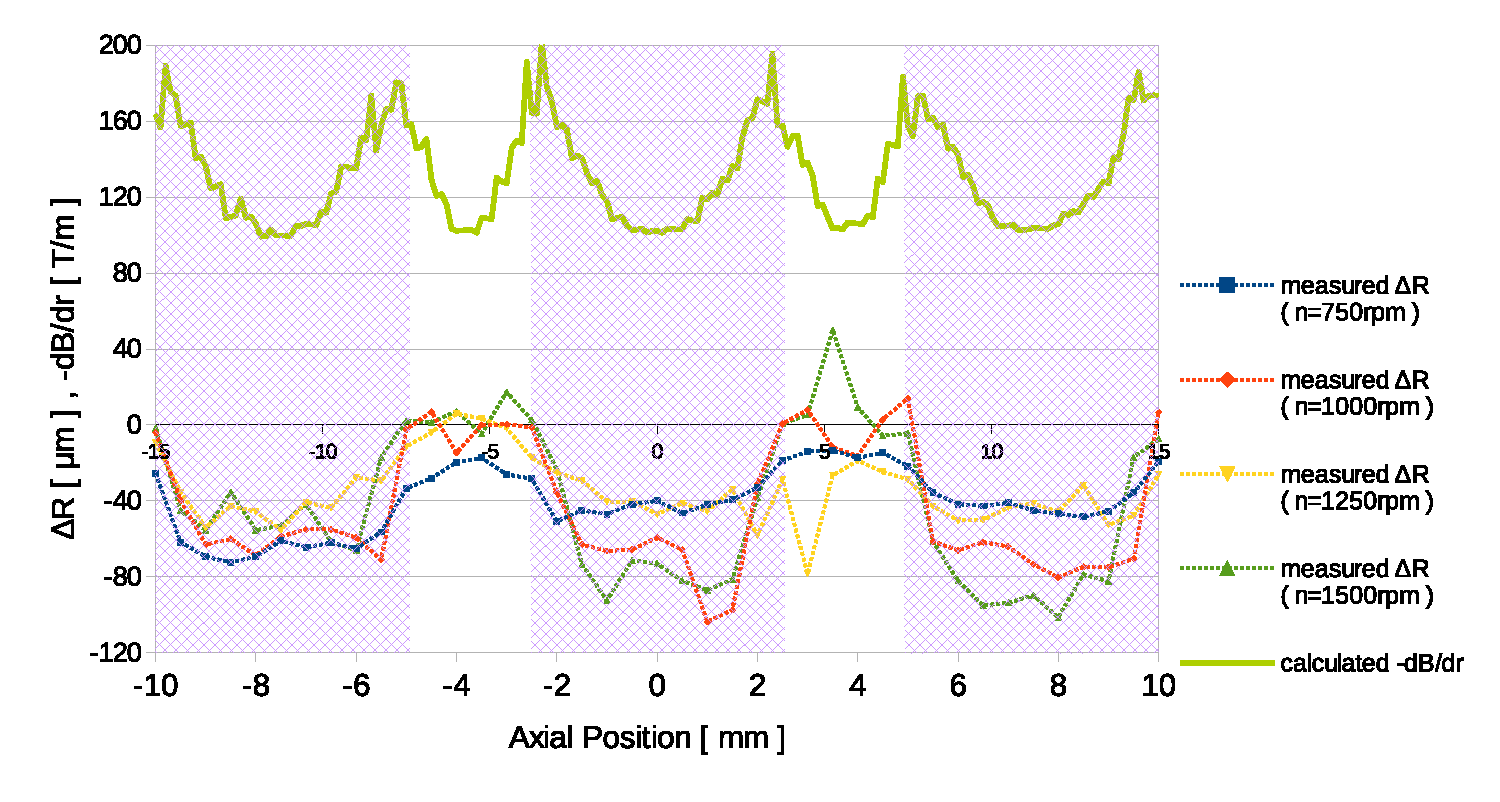
\includegraphics[width=150mm]{Typealpha_dB.eps}
    \end{center}
    \caption{研磨加工による内径変化と磁束密度の勾配(Type$\alpha$)}
    \label{fig:Typealpha_dB}
  \end{figure}

  \begin{figure}[H]
    \begin{center}
      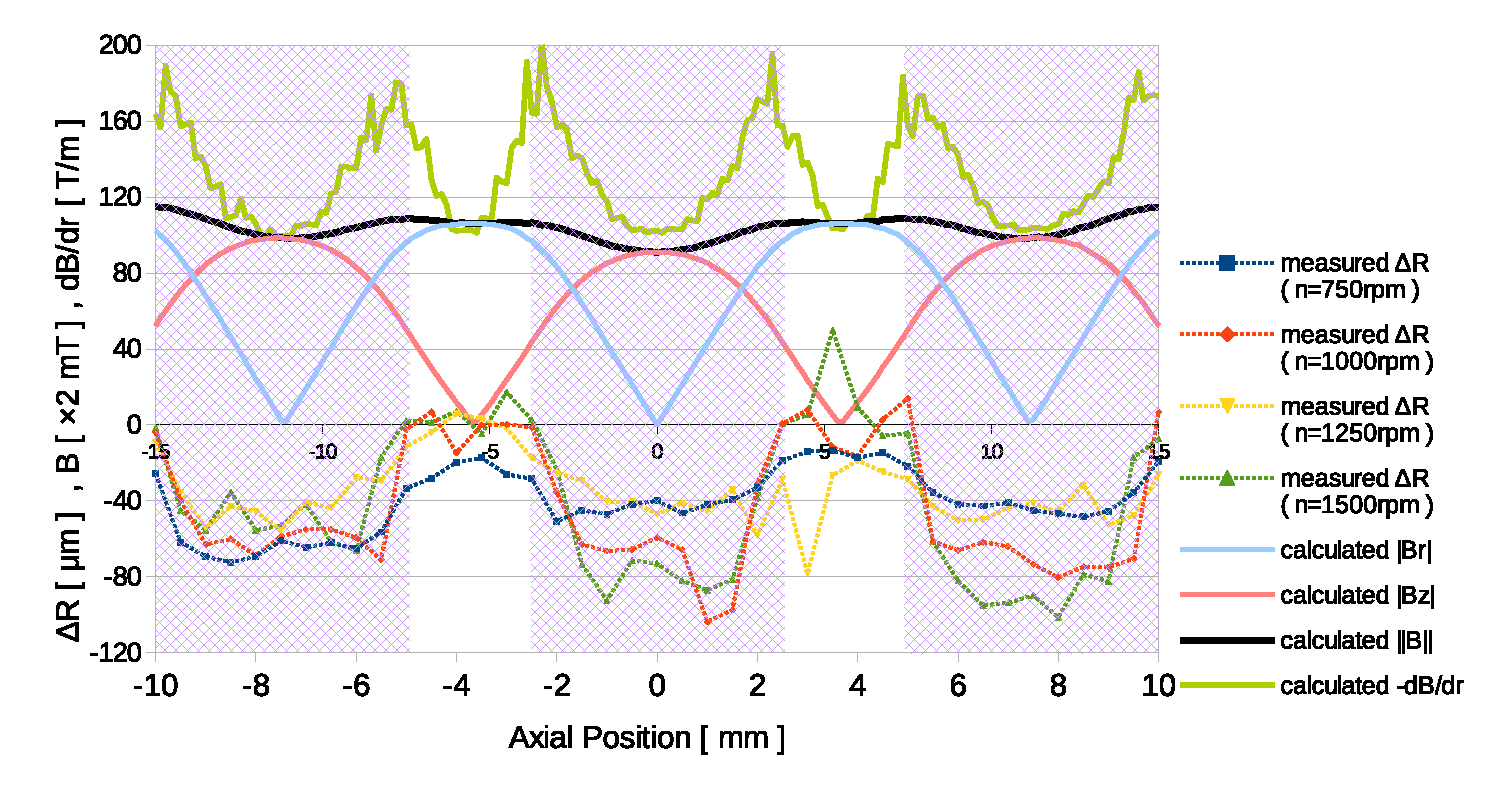
\includegraphics[width=150mm]{Typealpha.eps}
    \end{center}
    \caption{研磨加工による内径変化と磁場諸量(Type$\alpha$)}
    \label{fig:Typealpha}
  \end{figure}


  \begin{table}[H]
    \begin{tabular}{|c|r|r|r|r|} \hline 
         Type$\alpha$ & 750rpm & 1000rpm & 1250rpm & 1500rpm \\ \hline
         $B_r$ & -0.65 & -0.74  & -0.54 & -0.80 \\ \hline
         $B_z$ & 0.81 & 0.82 & 0.62 & 0.87 \\ \hline
         $B$ & -0.34 & -0.57 & -0.34 & -0.63 \\ \hline
    \end{tabular}
    \centering
    \caption{相関係数(Type$\alpha$)}
    \label{tab:CC_alpha}
  \end{table}


  \begin{figure}[H]
    \begin{center}
      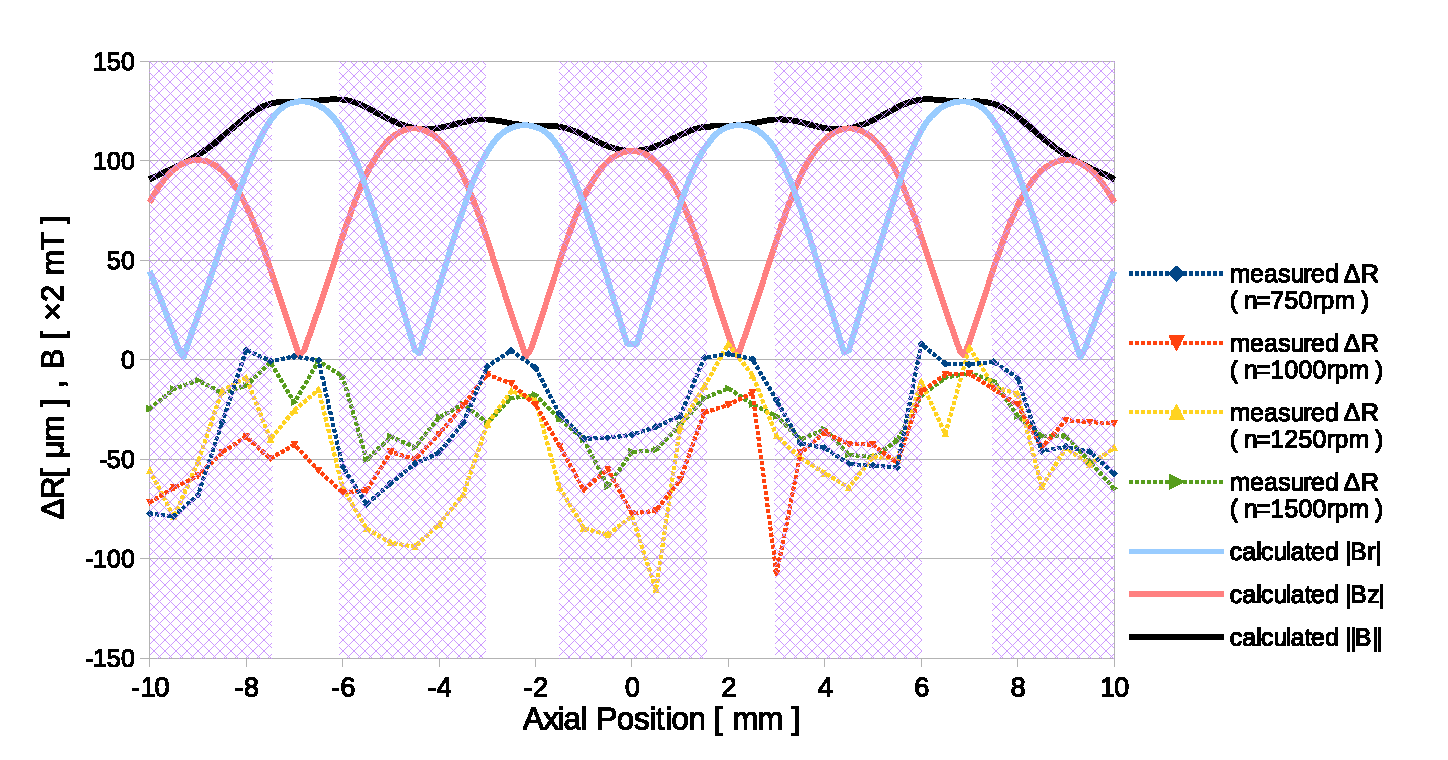
\includegraphics[width=150mm]{Typebeta_B.eps}
    \end{center}
    \caption{研磨加工による内径変化と磁束密度(Type$\beta$)}
    \label{fig:Typebeta_B}
  \end{figure}

  \begin{figure}[H]
    \begin{center}
      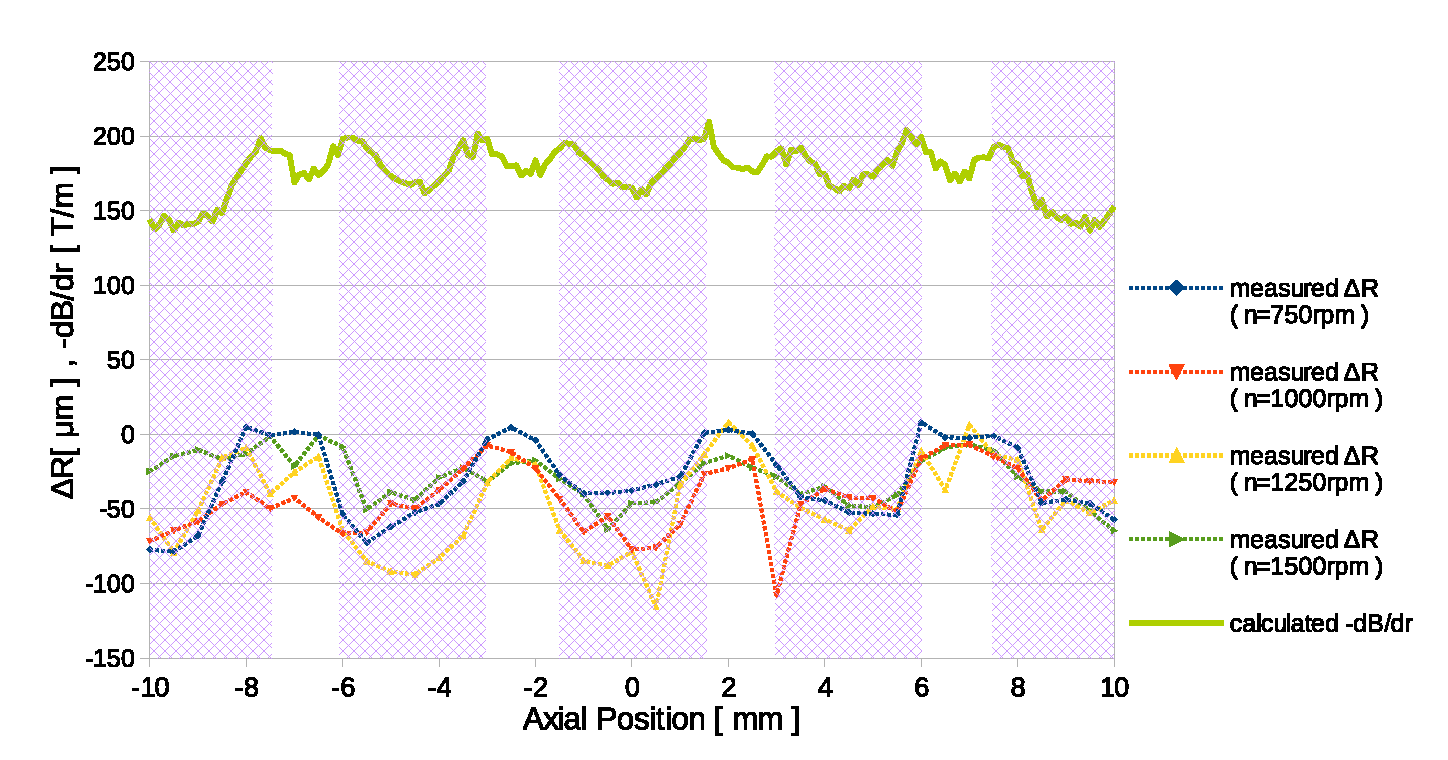
\includegraphics[width=150mm]{Typebeta_dB.eps}
    \end{center}
    \caption{研磨加工による内径変化と磁束密度の勾配(Type$\beta$)}
    \label{fig:Typebeta_dB}
  \end{figure}

  \begin{figure}[H]
    \begin{center}
      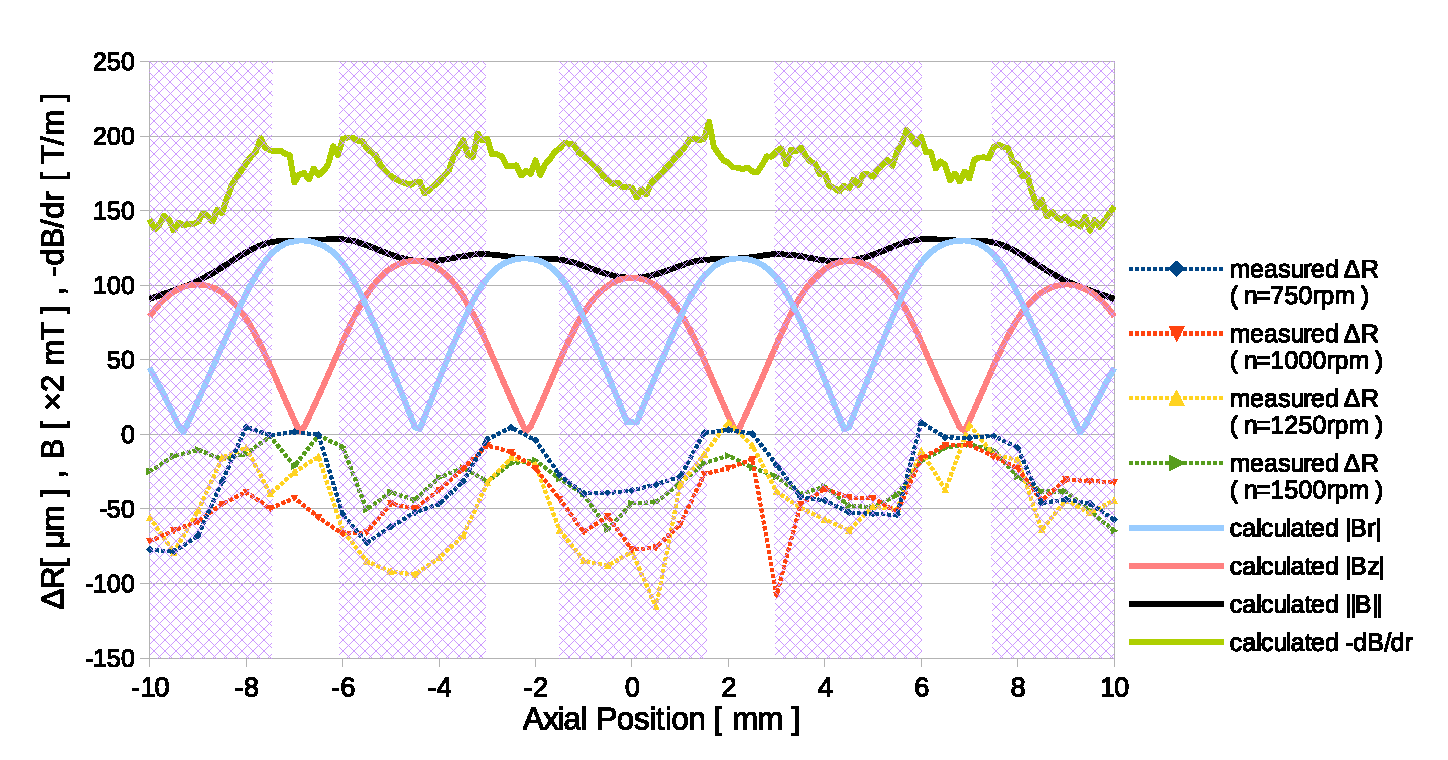
\includegraphics[width=150mm]{Typebeta.eps}
    \end{center}
    \caption{研磨加工による内径変化と磁気諸量(Type$\beta$)}
    \label{fig:Typebeta}
  \end{figure}

  \begin{table}[H]
    \begin{tabular}{|c|r|r|r|r|} \hline 
         Type$\beta$ & 750rpm & 1000rpm & 1250rpm & 1500rpm \\ \hline
         $B_r$ & -0.77 & -0.38 & -0.67 & -0.64 \\ \hline
         $B_z$ & 0.78 & 0.42 & 0.71 & 0.63 \\ \hline
         $B$ & -0.52 & -0.30 & -0.38 & -0.50 \\ \hline
    \end{tabular}
    \centering
    \caption{相関係数(Type$\beta$)}
    \label{tab:CC_beta}
  \end{table}

  \subsection{解析結果と加工実験結果との比較まとめ}
磁束密度の大きさと加工量との間に関連性を見出すことはできなかった. 同様に磁束密度の大きさと加工量との間についても関連性がないことが分かった. これら2つはネガティブな結果であって, これまでの実験結果と解析結果との比較のみでは加工原理への直接的な理解へは至ることができないと言えた. 

  \subsection{鉄粉に働く力の概算}\label{iron_F}
工具Type$\alpha$について磁石側面から1mmの位置での磁束密度の大きさと勾配を用いて, MCFに含まれる鉄粉に働く様々な力を概算し評価した. 鉄粉に働く磁力$f_{grav}$, 遠心力$f_{cent}$, 重力$f_{mag}$について体積あたりの力{\rm N/$m^3$}の概算結果を可視化し, 常用対数スケールで表したものを図\ref{fig:approx}に示す. また計算式と具体的な計算結果についても式\ref{eq:grav}, 式\ref{eq:cent}, 式\ref{eq:mag}に示し, 表\ref{tab:iron_tool}, 表\ref{tab:physical_constant}に計算の際に必要な諸量をまとめた. \par
鉄粉に働く重力や遠心力と比較して磁力が支配的であることから, 磁気的な効果のみを考えた本シミュレーションの妥当性が間接的に確認できる. 

\begin{comment}
 まず鉄粉の体積に関して, 
      \begin{eqnarray}
        v & = & \frac{4\pi (\frac{R}{2})^3  }{3} \nonumber \\ 
          & = & \frac{\pi R^3}{6}  \\ 
      \end{eqnarray} 
\end{comment}

      \begin{eqnarray}
        f_{grav} & = & \rho g\nonumber \\
                 & = & (7.86\times10^3) \times 9.8 {\rm [N/m^3]}\nonumber \\ 
              f   & = & 7.70 \times 10^4 {\rm [N/m^3]}, \label{eq:grav} \\ \nonumber  \\
\begin{comment}
        F_{grav} & = & m g \nonumber \\ 
                 & = & \frac{ \rho \pi d^3 g }{6} \nonumber \\
                 & = & \frac{ (7.86\times10^3) \times \pi \times (1.2\times10^{-6})^3 \times 9.8 }{6} [N]\nonumber \\ 
                 & = & 6.97 \times 10^{-14} [N], \\ \nonumber \\
\end{comment}
        f_{cent} & = & \frac{ \rho R \omega^2 }{2}\nonumber \\
                 & = & \frac{ (7.86\times10^3) \times (15\times10^{-3}) \times (\frac{1000\times2\pi}{60})^2 }{2} {\rm [N/m^3]}\nonumber \\
                 & = & 6.46 \times 10^5 {\rm [N/m^3] }, \label{eq:cent} \\ \nonumber  \\
\begin{comment}
        F_{cent} & = & \frac{m R \omega^2 }{2} \nonumber \\
                 & = & \frac{ \rho \pi d^3 R \omega^2 }{12}\nonumber \\
                 & = & \frac{ (7.86\times10^3) \times \pi \times (1.2\times10^{-6})^3 \times (15\times10^{-3}) \times (\frac{1000\times2\pi}{60})^2 }{12} [N]\nonumber \\
                 & = & 5.85 \times 10^{-13} [N], \\ \nonumber \\
\end{comment}
        f_{mag} & = & \bm{M} \cdot \nabla \bm{H} \nonumber \\
                & = & \mu_0 \chi \bm{H} \cdot \nabla \bm{H} \nonumber \\
                & = & (4\pi \times 10^{-7}) \times 2000 \times (1.6\times10^5) \times (1.1\times10^8) {\rm [N/m^3]} \nonumber \\
                & = & 4.83 \times 10^{10} {\rm [N/m^3]}. \label{eq:mag} 
\begin{comment}
        F_{mag} & = & - v \bm{M} \cdot \nabla \bm{H} \nonumber \\
                & = & - \frac{ \mu_0 \pi d^3 \chi \bm{H} \cdot \nabla \bm{H} }{6}  \nonumber \\
                & = & - \frac{ (4\pi \times 10^{-7}) \times \pi \times (1.2\times10^{-6})^3 \times 2000 \times (1.6\times10^5) \times (1.2\times10^8) }{6} [N] \nonumber \\
                & = & - 4.36 \times 10^{-8}[N].
\end{comment}
      \end{eqnarray} 

\begin{comment}
    \subsubsection{砥粒について}
 式\ref{grav},\ref{cent},\ref{mag},表\ref{tab:tab2}より砥粒にはたらく力$f^{abr}$は, 
      \begin{eqnarray}
        f^{abr}_{grav} & = & \rho g\nonumber \\
                        & = & (3.4\times10^3) \times 9.8 [N/m^3]\nonumber \\ 
                        & = & 3.33 \times 10^4 [N/m^3], \\ 
        F^{abr}_{grav} & = & \frac{ \rho \pi d^3 g }{6} \nonumber \\
                        & = & \frac{ (3.4\times10^3) \times \pi \times (3\times10^{-6})^3 \times 9.8 }{6} [N]\nonumber \\ 
                        & = & 4.71 \times 10^{-13} [N], \\ \nonumber \\
        f^{abr}_{cent} & = & \frac{ \rho R \omega^2 }{2}\nonumber \\
                        & = & \frac{ (3.4\times10^3) \times (15\times10^{-3}) \times (\frac{1000\times2\pi}{60})^2 }{2}[N/m^3]\nonumber \\
                        & = & 2.80 \times 10^5 [N/m^3], \\ 
        F^{abr}_{cent} & = & \frac{ \rho \pi d^3 R \omega^2 }{12}\nonumber \\
                        & = & \frac{ (3.4\times10^3) \times \pi \times (3\times10^{-6})^3 \times (15\times10^{-3}) \times (\frac{1000\times2\pi}{60})^2 }{12} [N] \nonumber \\
                        & = & 3.95 \times 10^{-12} [N] , \\ \nonumber \\
        f^{abr}_{mag} & = & - \mu_0 \chi \bm{H} \cdot \nabla \bm{H} \nonumber \\
                       & = & - (4\pi \times 10^{-7}) \times (-0.098) \times (1.6\times10^5) \times (1.2\times10^8) [N/m^3] \nonumber \\
                       & = & 2.36 \times 10^6 [N/m^3], \\
        F^{abr}_{mag} & = & - \frac{ \mu_0 \pi d^3 \chi \bm{H} \cdot \nabla \bm{H} }{6}  \nonumber \\
                       & = & - \frac{ (4\pi \times 10^{-7}) \times \pi \times (3\times10^{-6})^3 \times (-0.098) \times (1.6\times10^5) \times (1.2\times10^8) }{6} [N]\nonumber \\
                       & = & 3.34 \times 10^{-11} [N].
      \end{eqnarray}
\end{comment}

  \begin{figure}[H]
    \begin{center}
      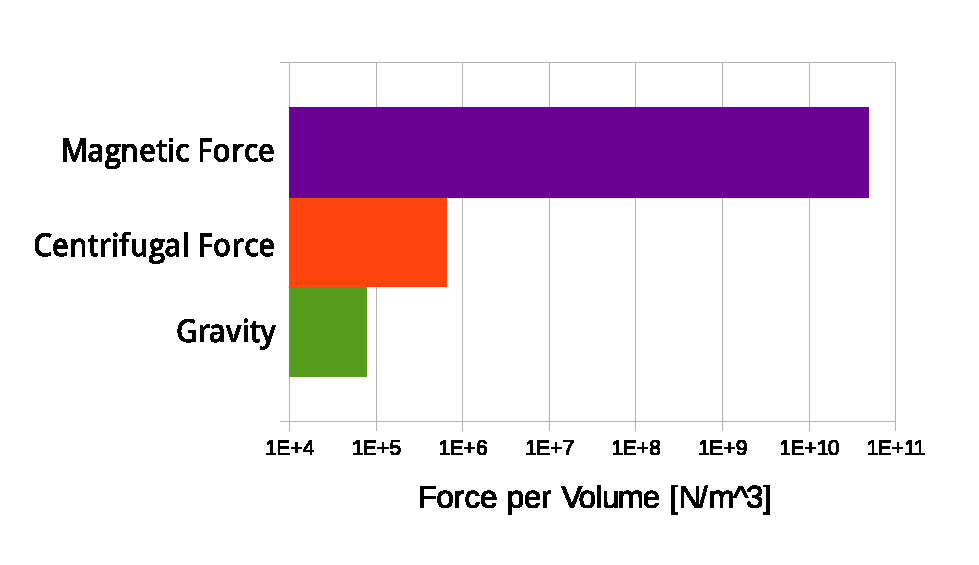
\includegraphics[width=100mm]{approx.eps}
    \end{center}
    \caption{磁性体粒子に働く力の概算}
    \label{fig:approx}
  \end{figure}

\begin{comment}
  \begin{table}[htb]
    \begin{tabular}{|l|c|l|c|} \hline 
         工具外径R[mm] & 15 & 工具回転数[rpm] & 1000 \\ \hline
         磁場の強さH[A/m] & $1.6\times10^5$ & 磁場の強さの勾配$\nabla H[A/m^2]$ & $1.8\times10^8$ \\ \hline
         外径(鉄粉)$d^{iron}[\mu m]$ & $1.2$ & 外径(砥粒)$d^{abr}[\mu m]$ & $3$ \\ \hline
         密度(鉄粉)$\rho^{iron}[g/cm^3]$ & $7.86$ & 密度(砥粒)$\rho^{abr}[g/cm^3]$ & $3.4$  \\ \hline
         磁化率(鉄粉)$\chi^{iron}$ & $2000$ & 磁化率(砥粒)$\chi^{abr}$ & $-0.098$  \\ \hline
    \end{tabular}
    \centering
    \label{tab:MCF_table}
    \caption{MCF諸元}
  \end{table}
\end{comment}

  \begin{table}[H]
    \begin{tabular}{|l|c|l|c|} \hline 
       Tool Type & $\alpha$ & External Radius {\it R}[mm] & 15 \\ \hline
       Intensity of Magnetic field {\it H}[A/m] & $1.6\times10^5$ & Partial Derivative $-\frac{\partial H}{\partial r}$ & $1.1\times10^8$ \\ \hline
       Number of Revolution [rpm] & 1000 & Magnetic Susceptibity $\chi$ & $2000$   \\ \hline
       Particle Size {\it d}[$\mu$m] & $1.2$ & Density {\rm $\rho[g/cm^3]$ } & $7.86$   \\ \hline
    \end{tabular}
    \centering
    \caption{鉄粉および工具諸元}
    \label{tab:iron_tool}
  \end{table}

  \begin{table}[H]
    \begin{tabular}{|c|c||c|c|} \hline
      Gravitational Acceleration {\it g}[m/$s^2$] & 9.8 & Permeability of Vacuum $\mu_0$[H/m] & $4\pi\times10^{-7}$ \\ \hline
    \end{tabular}
    \centering
    \caption{物理定数}
    \label{tab:physical_constant}
  \end{table}

\newpage

\section{様々な寸法の工具についての体系的な解析}
前章で述べたようにこれまでの加工実験結果と磁場解析結果との比較では加工原理への直接的な理解には不十分であることが分かった. \par
ここで原理への理解を深めるために解析結果との比較を前提として適切な実験工具を設計できないか考える. もし様々な寸法の工具について網羅的に計算を行いそれぞれ比較を行えるならば, それにのっとって適切な工具の設計を行うことができる. この観点から本研究では網羅的な解析システムを構築した. 

  \subsection{実験工具の設計}
研磨においてある磁気的な特性が加工原理への考察で重要な役割を果たすと予想されるとき, 適切に工具を設計することでその特性が加工量の空間分布に著しい影響を与えるような工具を, 本システムでは設計することができる. この工具を用いた加工実験は実際にその予想が正しいかどうか検証するのに便利である. またいくつかの磁気的な特性のうちどれがもっとも寄与が大きいかなどを考える際にも, 本システムを適用することができる. 

  \subsection{解析結果の応用}
磁気機能性流体とは一般に磁場のもとで機能性をもつ流体の総称であり, 磁気混合流体(MCF)もこれに含まれる. これは逆に磁場のごく小さな領域ではその機能性を持たないとも言える. これから磁束密度がごく小さな領域が大きいような特性をもつ工具は応用上重要ではないことが予想される. この観点から研磨を行う領域で磁束密度があるしきい値を下回るかどうかについて評価を行う. 図\ref{fig:B_app}に例として磁石の間隔を変えた際の磁束密度の分布と磁束密度のしきい値について示した. 今回の磁束密度のしきい値は0.18T程度としたが, これは実験的におおよその値を見積ったものである. \cite{塚田}\par
図から磁束密度の大きさに関して0.18Tを下回っている領域がある工具が存在することがわかる. この工具について磁気機能性流体の応用上は重要でないとして, 工具設計の際の考察の対象から除外することができる. すなわち本システムでは, 磁束密度の大きさにあるしきい値を設定しそのしきい値を下回る領域が大きな工具について実用上は重要でないとして除外し, 設計する工具に関して絞り込みを行うことができる. 

  \begin{figure}[H]
    \begin{center}
      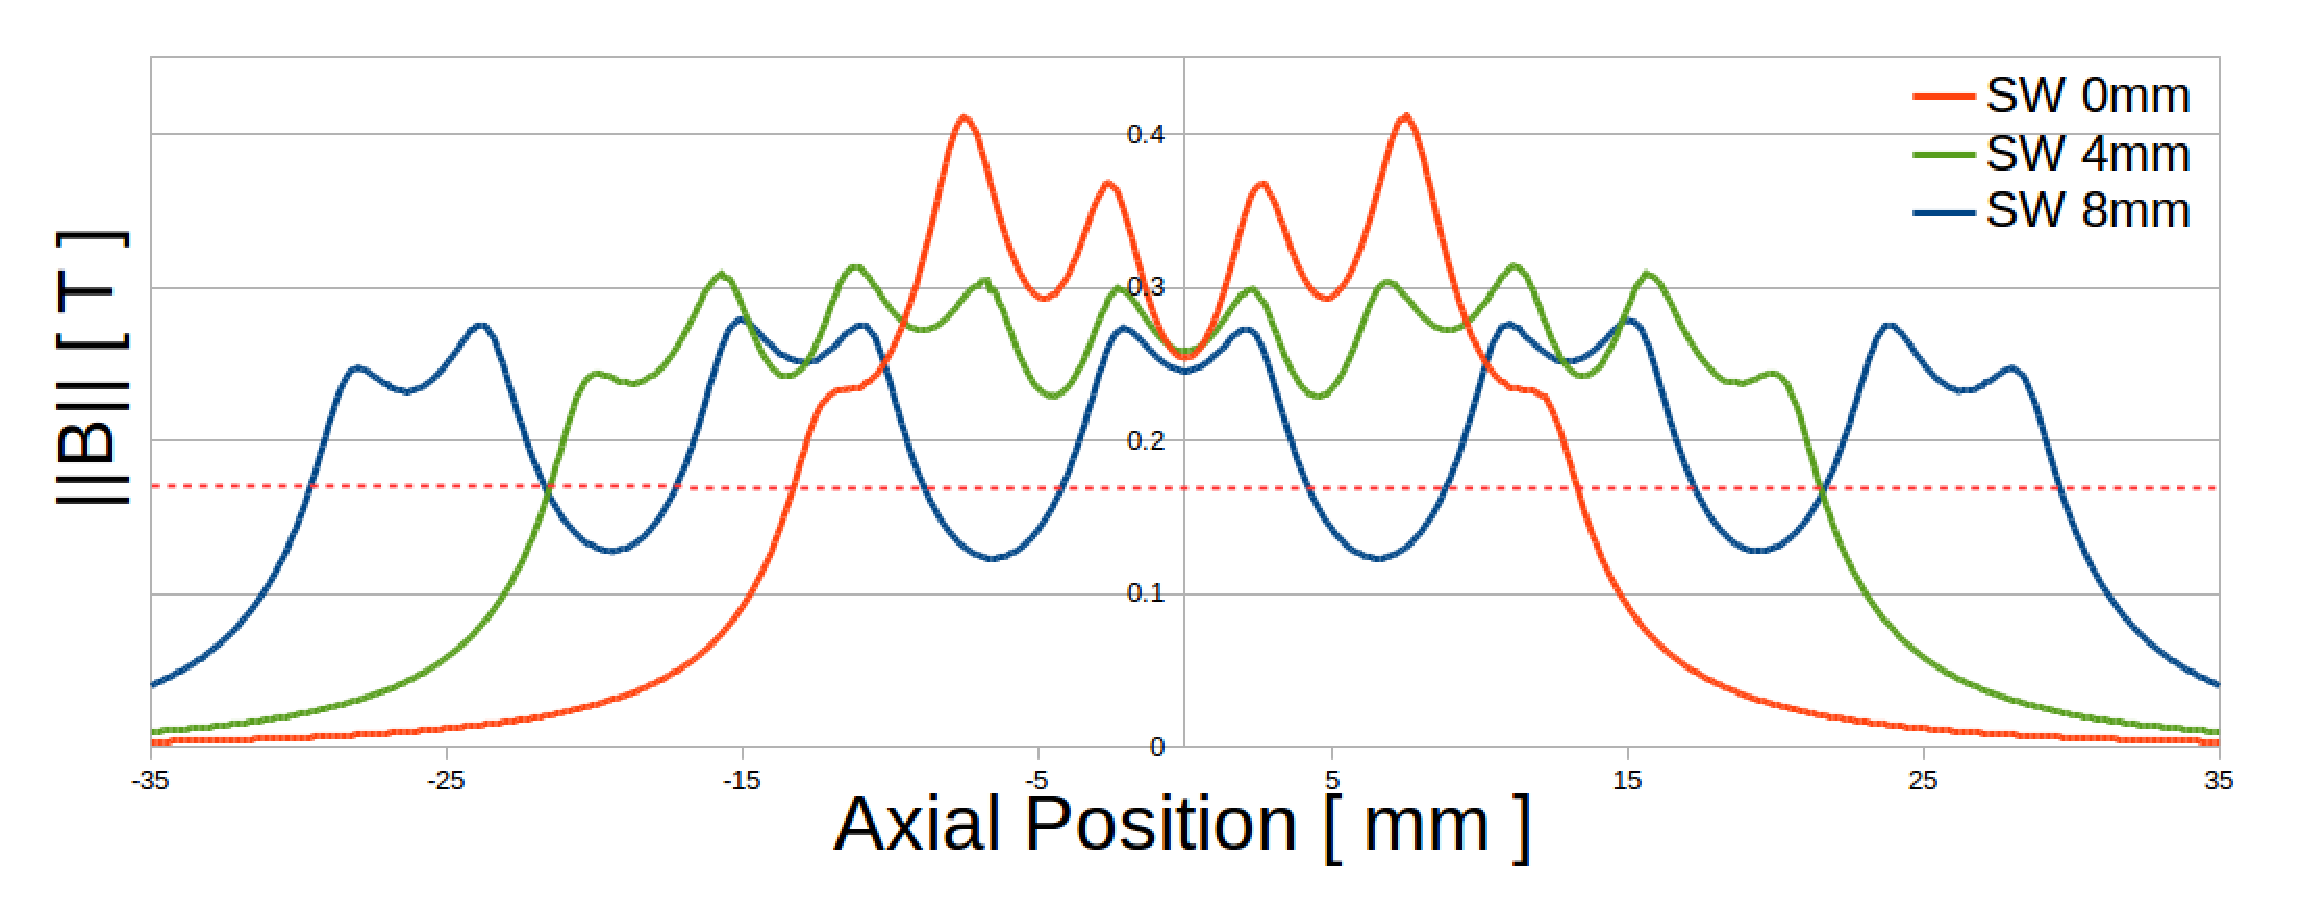
\includegraphics[width=125mm]{B_app.eps}
    \end{center}
    \caption{解析結果の応用}
    \label{fig:B_app}
  \end{figure}

  \subsection{解析システム}
図\ref{fig:DFD}に解析システムのデータの流れを示す. このシステムでは解析パラメータの設定と計算, 基礎分析を自動で行うことができる. これによって様々な工具間での体系的な比較を行うことができるようになった. なお解析システムはDOA( Data Oriented Approach )にのっとって構成し, 塚田らの作成したシステム\cite{塚田}にくらべデータとプログラムについてそれぞれ再利用性を高くすることに成功した. 具体的には任意の位置での磁束密度分布とそれをもとにした解析量などを, 一括して後から取り出すことができるようにした. 解析可能なモデルについても前研究を引き継ぎ自由度の拡大を行ったことによって, 工具の幾何学的な自由度を網羅することができるようになった. プログラミングはおもにc言語をもちいて行っているが, Maxwell SVでの連続計算を行う際にはマクロ言語であるKMmacro\cite{KMmacro}, データの出力の際はMaxwell 2D PostProcess の内部マクロ, 解析結果の分析の際には一部R言語\cite{RR}を用いている. \par
表\ref{tab:tool_par}に計算を行った工具寸法パラメータについて示した. なおそれぞれの組み合わせをとるとのべ15000通り以上の工具形状になりうるが, そのすべてについて網羅的に解析を行った. 

  \begin{figure}[H]
    \begin{center}
      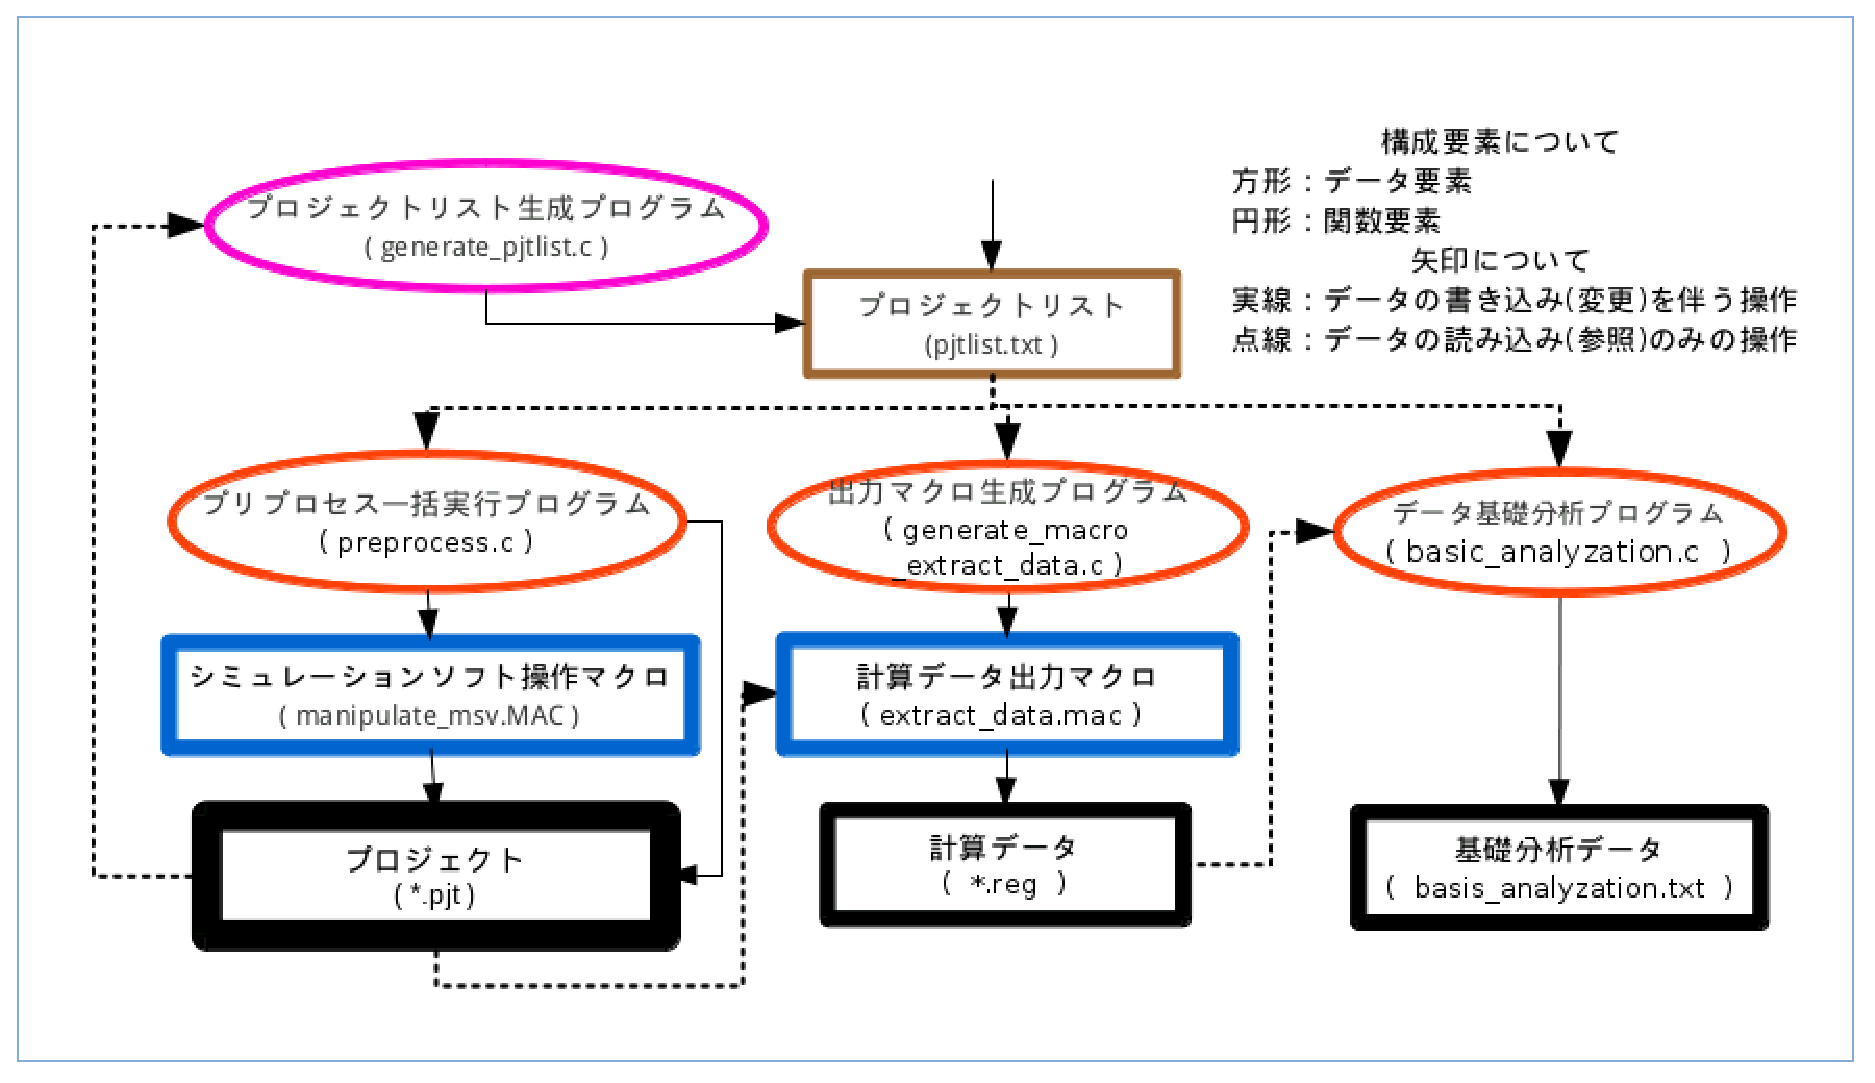
\includegraphics[width=125mm]{DFD.eps}
    \end{center}
    \caption{構成要素関連図(DFD: Data Flow Diagram)}
    \label{fig:DFD}
  \end{figure}

  \begin{table}[H]
    \begin{tabular}{|r||c|c|c|c|c|c|c|c|c|c|c|} \hline
        Number of Magnet & 3 & 4 & 5 & & & & & & & & \\ \hline 
        Width of Magnet [mm] & 3 & 4 & 5 & 6 & 7 & 8 & 9 & 10 & 11 & 12 & 13 \\ \hline
        Internal Diameter [mm] & 3 & 4 & 5 & 6 & 7 & 8 & 9 & 10 & 11 & & \\ \hline
        External Diameter [mm] & 6 & 7 & 8 & 9 & 10 & 11 & 12 & 13 & 14 & 15 &\\ \hline
        Width of Spacer [mm] & 1 & 2 & 3 & 4 & 5 & 6 & 7 & & & & \\ \hline
    \end{tabular}
    \centering
    \caption{工具寸法のとりうる値}
    \label{tab:tool_par}
  \end{table}

  \subsection{工具の形状による磁束密度の特性への一般的な考察}
次に円管内面における磁束密度の大きさの分布について, 解析値のグラフへの可視化を行った. 円管内面研削での工具形状については, 磁石の個数を含めて, 磁石の厚さ, 内半径, 外半径, スペーサの厚さ, 合わせて5つのパラメータが存在する. また被加工管の内半径も工学的な要請にあわせて変化しうるので, データの取り出しの際に適切に設定を行った. これら合わせて6つのパラメータの変化に対し磁束密度の大きさの分布への考察を行った. \par
図\ref{fig:B_delta}に被加工管内半径(磁石外側面との距離)を変化させた際の磁束密度分布を示した. 磁石外側面との距離が小さくなるほど磁束密度は一般に大きく, 磁極周辺での極大が特に鋭くなり磁石なかほどと磁石の間での極小もはっきりと分かる. これは磁極との距離が小さくなるためだと考えられる. \par
図\ref{fig:B_mn}に工具に用いる磁石の個数を変化させた際の磁束密度分布を示した. 軸方向位置が2.5mm付近では磁石の個数が1つの場合では磁束密度が0.25T程度であるのに対して, 3つや5つの場合では0.3T程度と磁束密度が20\%程度大きくなっていることが分かる. しかし磁石の個数が3つと5つの場合を比較しても大きな差はないことが言える. したがって磁石の間で磁極が対向している領域周辺では磁束線が互いに反発しあい, 磁束密度の大きさが磁石が単独で存在しているときに比べ大きくなっていることが確認できた. \par
図\ref{fig:B_ir}に磁石の内半径を変化させた際の磁束密度分布を示した. 内半径が小さくなることで磁石の体積が大きくなり磁束密度も一般に大きくなることが分かる. \par
図\ref{fig:B_mw}に磁石の厚さを変化させた際の磁束密度分布を示した. 磁石の厚さが大きくなると, 磁石の体積が大きくなり磁束密度の大きさは大きくなる. また磁石の厚さが小さくなると, それぞれの磁石なかほどに対応する領域に磁場の極小点が現れなくなる. 図\ref{fig:B_delta}でも, 工具磁石と被加工管内面との距離を大きくすると同様に磁石なかほどでの極小がはっきりとしなくなるため, 磁石なかほどで極小が存在するかどうかは磁石の幅に対する工具磁石と被加工管の距離の比に依存していることが考えられる. \par
図\ref{fig:B_sw}にスペーサの厚さを変化させた際の磁束密度分布を示した. スペーサの厚さが大きくなるにつれて磁束密度の大きさは小さくなり, 磁石が単独で存在する場合の磁束密度に近づく. スペーサの厚さが大きくなるとその中央での磁束密度の大きさは小さくなり, スペーサが存在しない場合磁束密度の大きさの極小点は存在しなくなる. 

  \begin{figure}[H]
    \begin{center}
      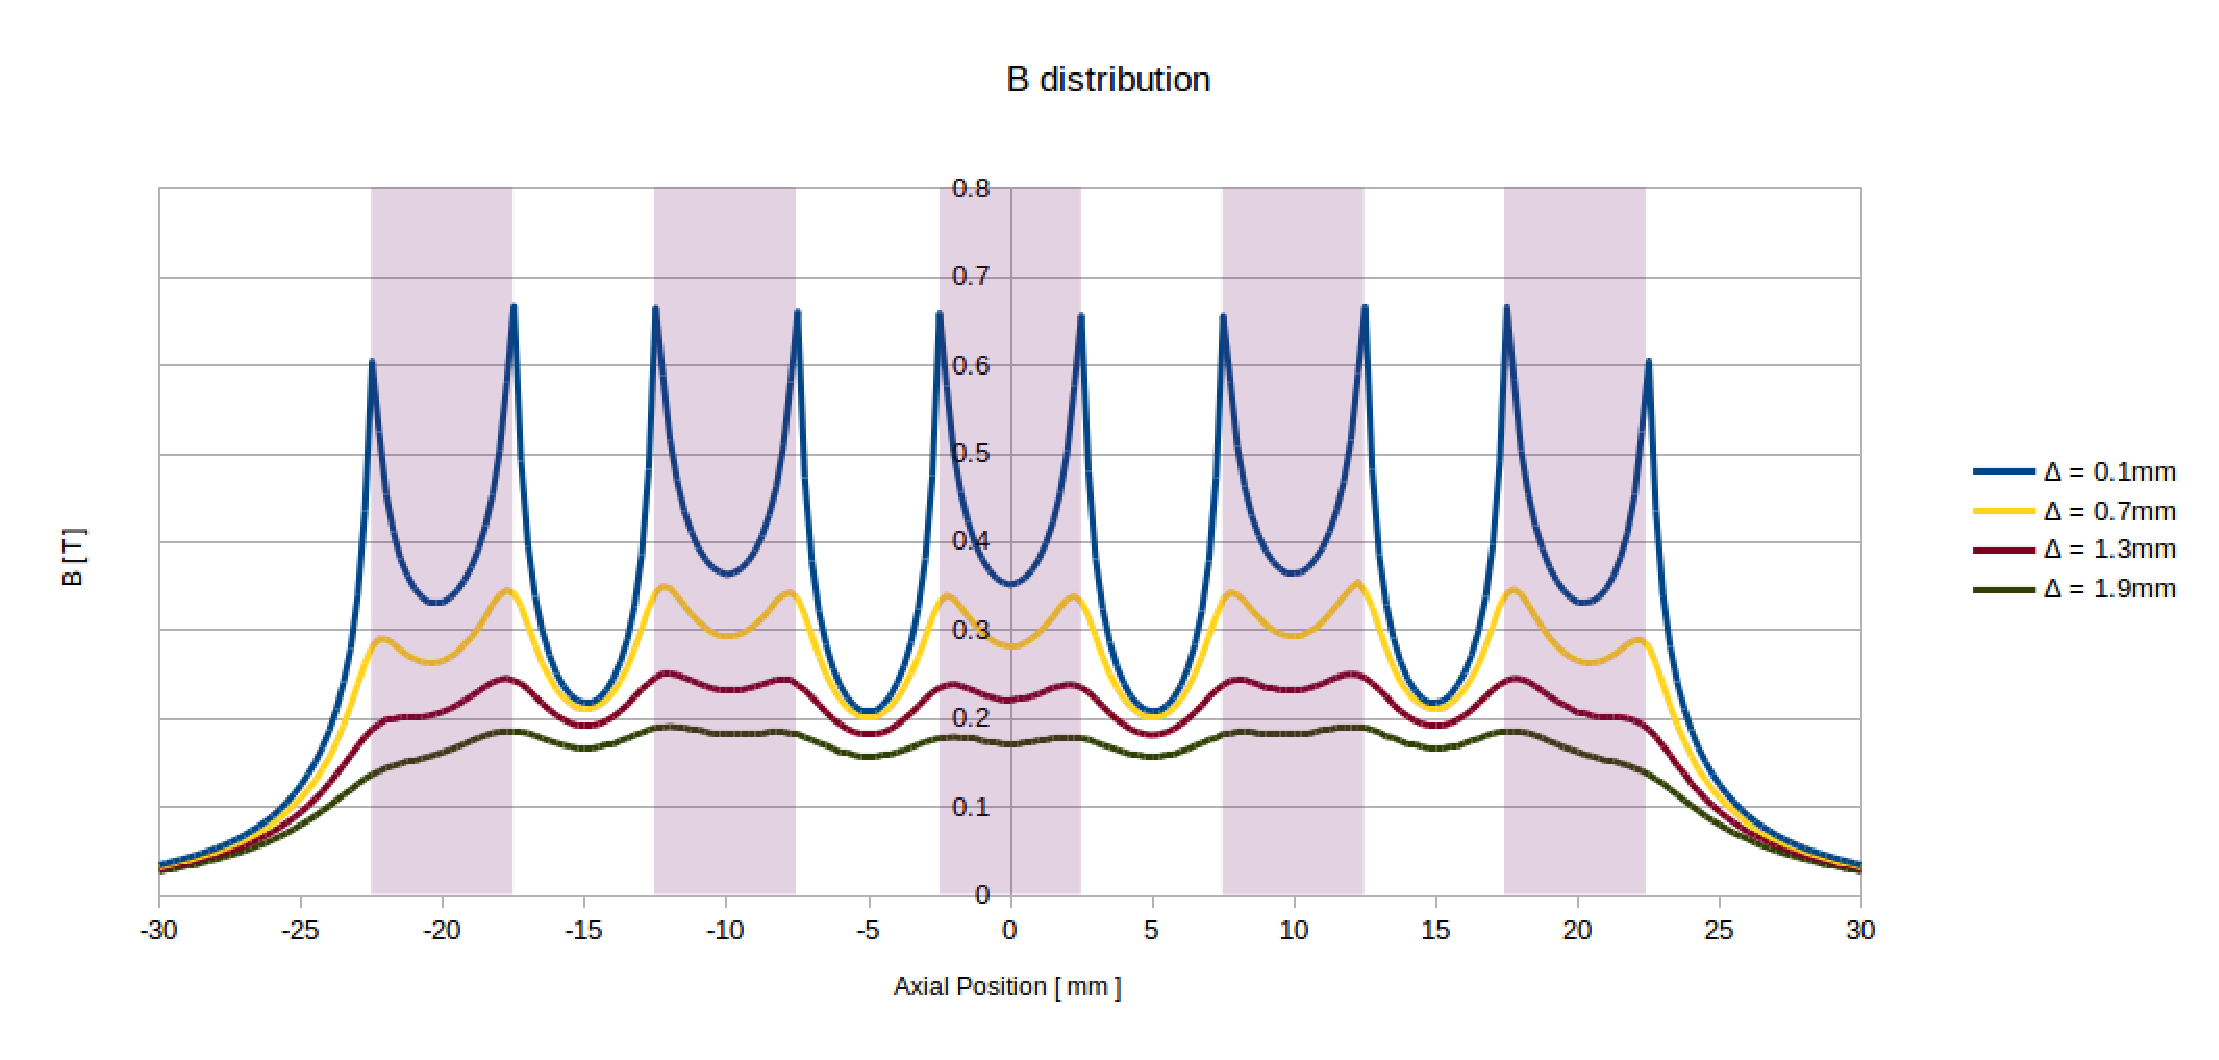
\includegraphics[width=125mm]{B_delta.eps}
    \end{center}
    \caption{被加工管内半径(磁石外側面との距離)を変化させた際の磁束密度の大きさの分布}
    \label{fig:B_delta}
  \end{figure}

  \begin{figure}[H]
    \begin{center}
      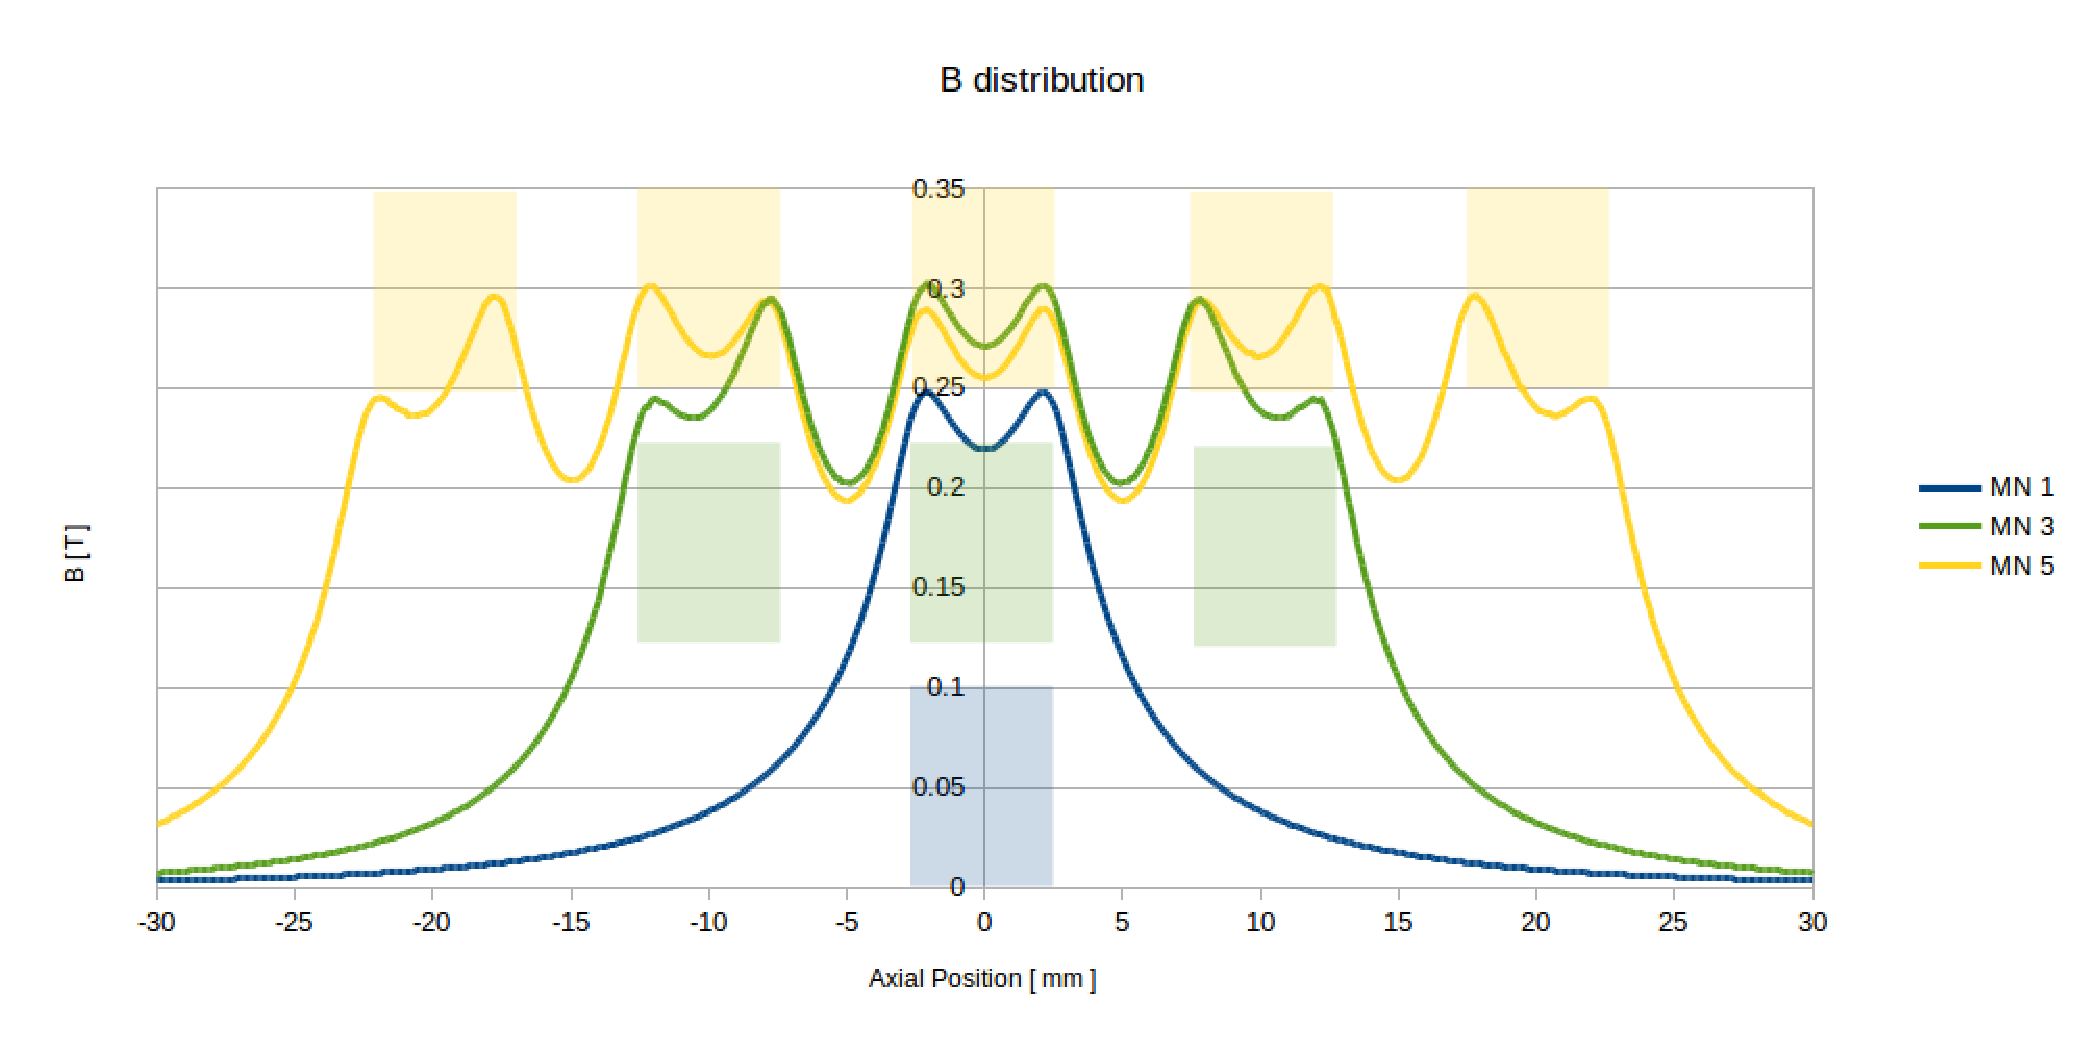
\includegraphics[width=125mm]{B_mn.eps}
    \end{center}
    \caption{磁石の個数を変化させた際の磁束密度の大きさの分布}
    \label{fig:B_mn}
  \end{figure}

  \begin{figure}[H]
    \begin{center}
      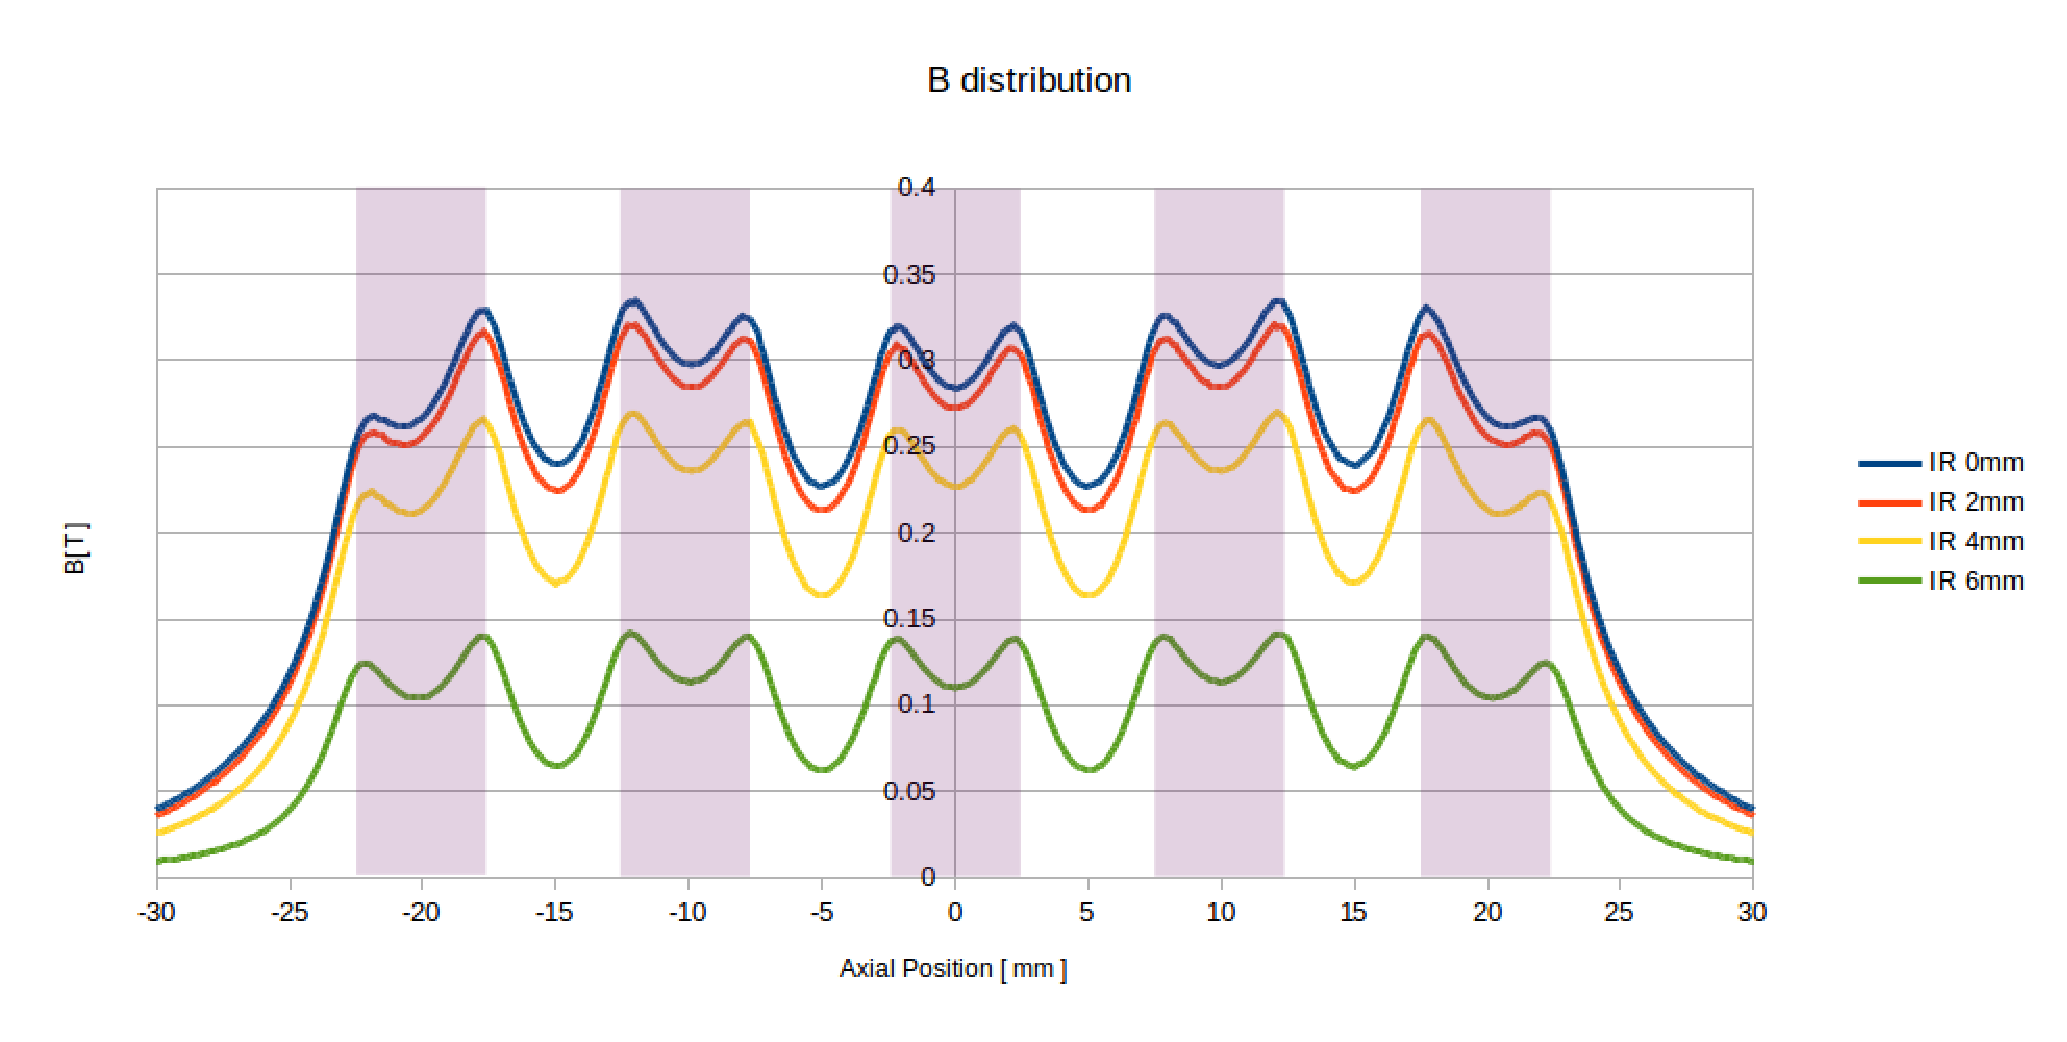
\includegraphics[width=125mm]{B_ir.eps}
    \end{center}
    \caption{磁石の内半径を変化させた際の磁束密度の大きさの分布}
    \label{fig:B_ir}
  \end{figure}

  \begin{figure}[H]
    \begin{center}
      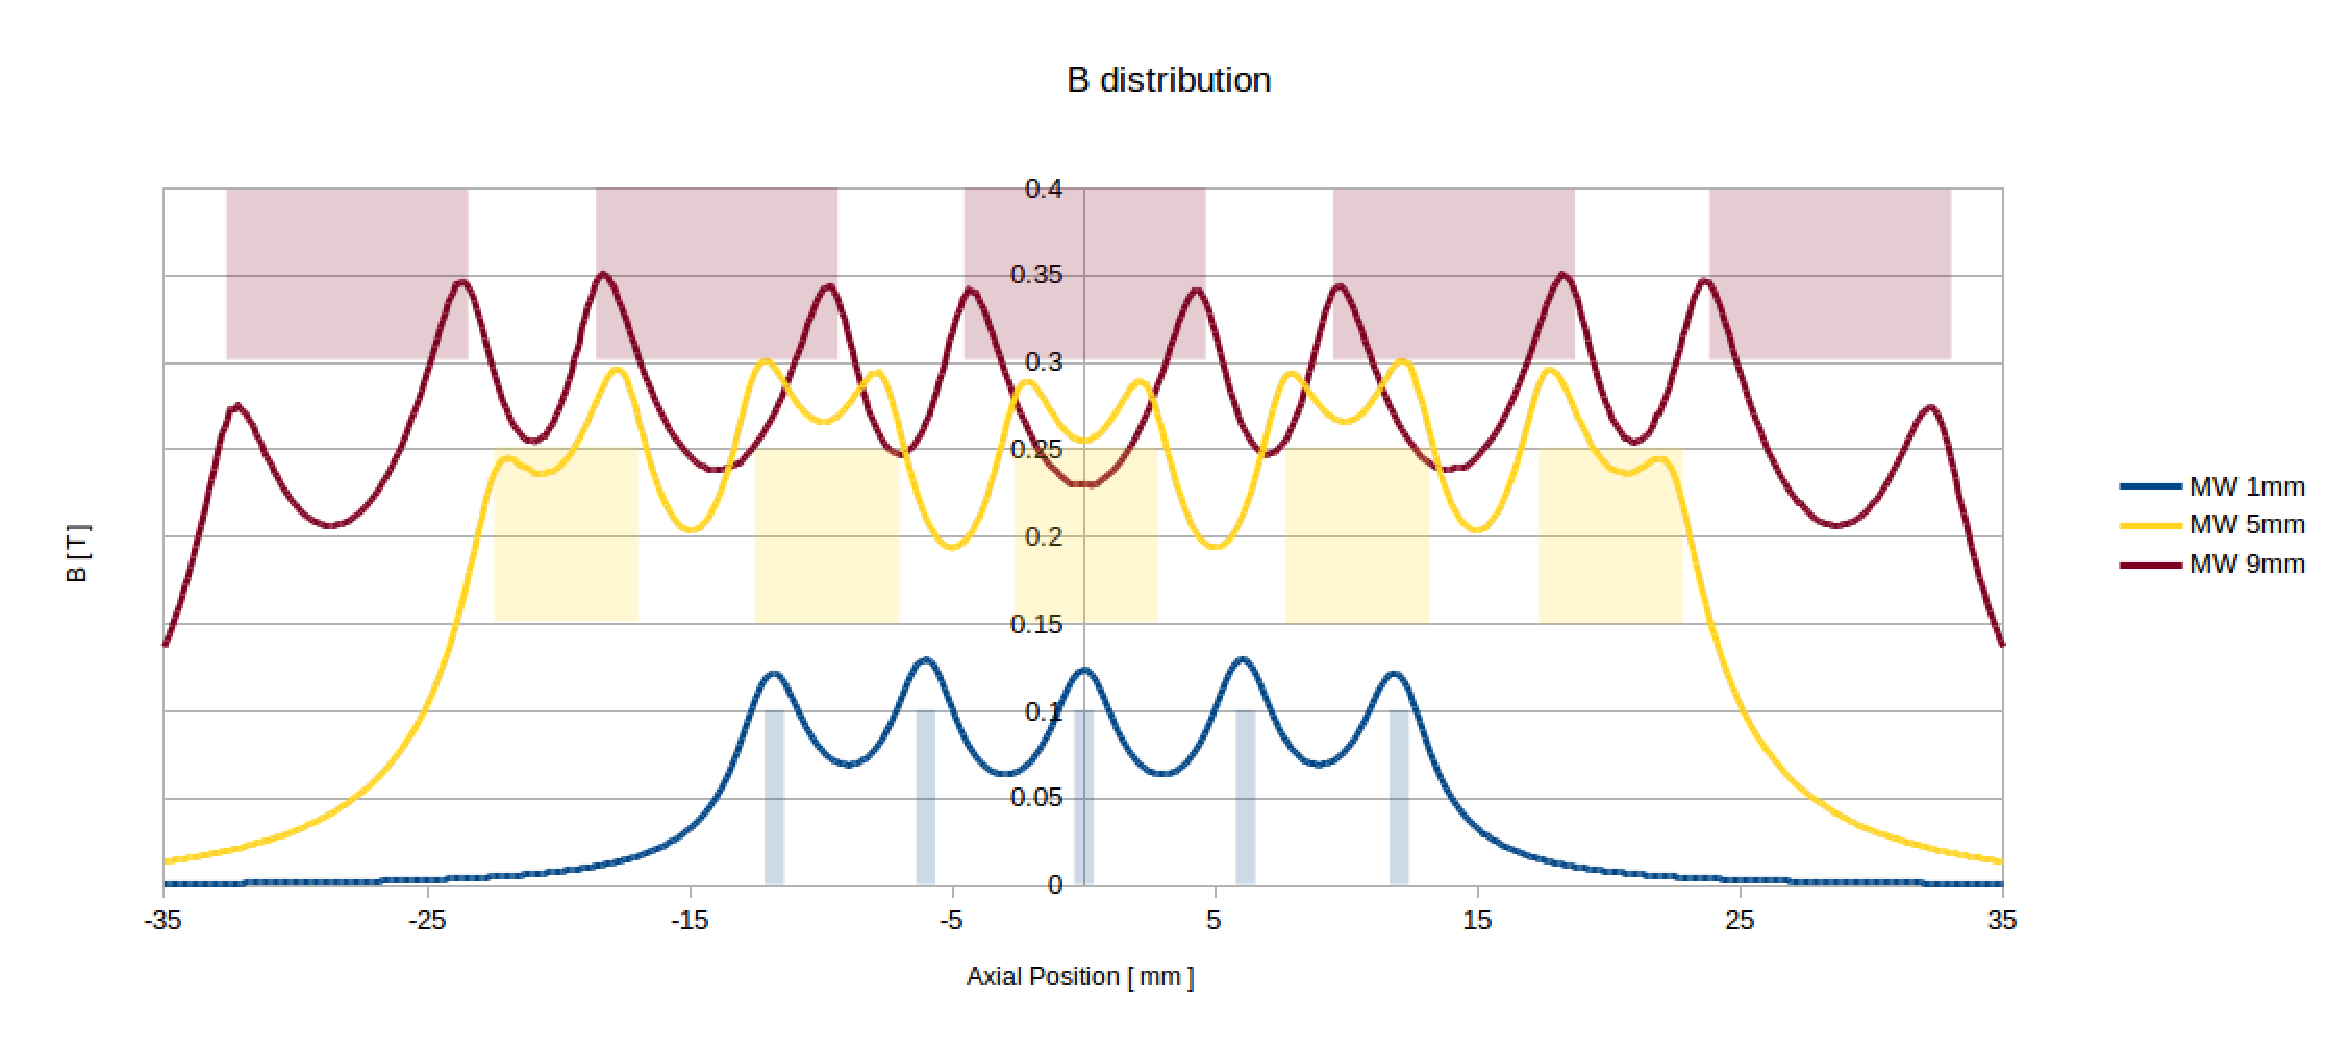
\includegraphics[width=125mm]{B_mw.eps}
    \end{center}
    \caption{磁石の幅を変化させた際の磁束密度の大きさの分布}
    \label{fig:B_mw}
  \end{figure}

  \begin{figure}[H]
    \begin{center}
      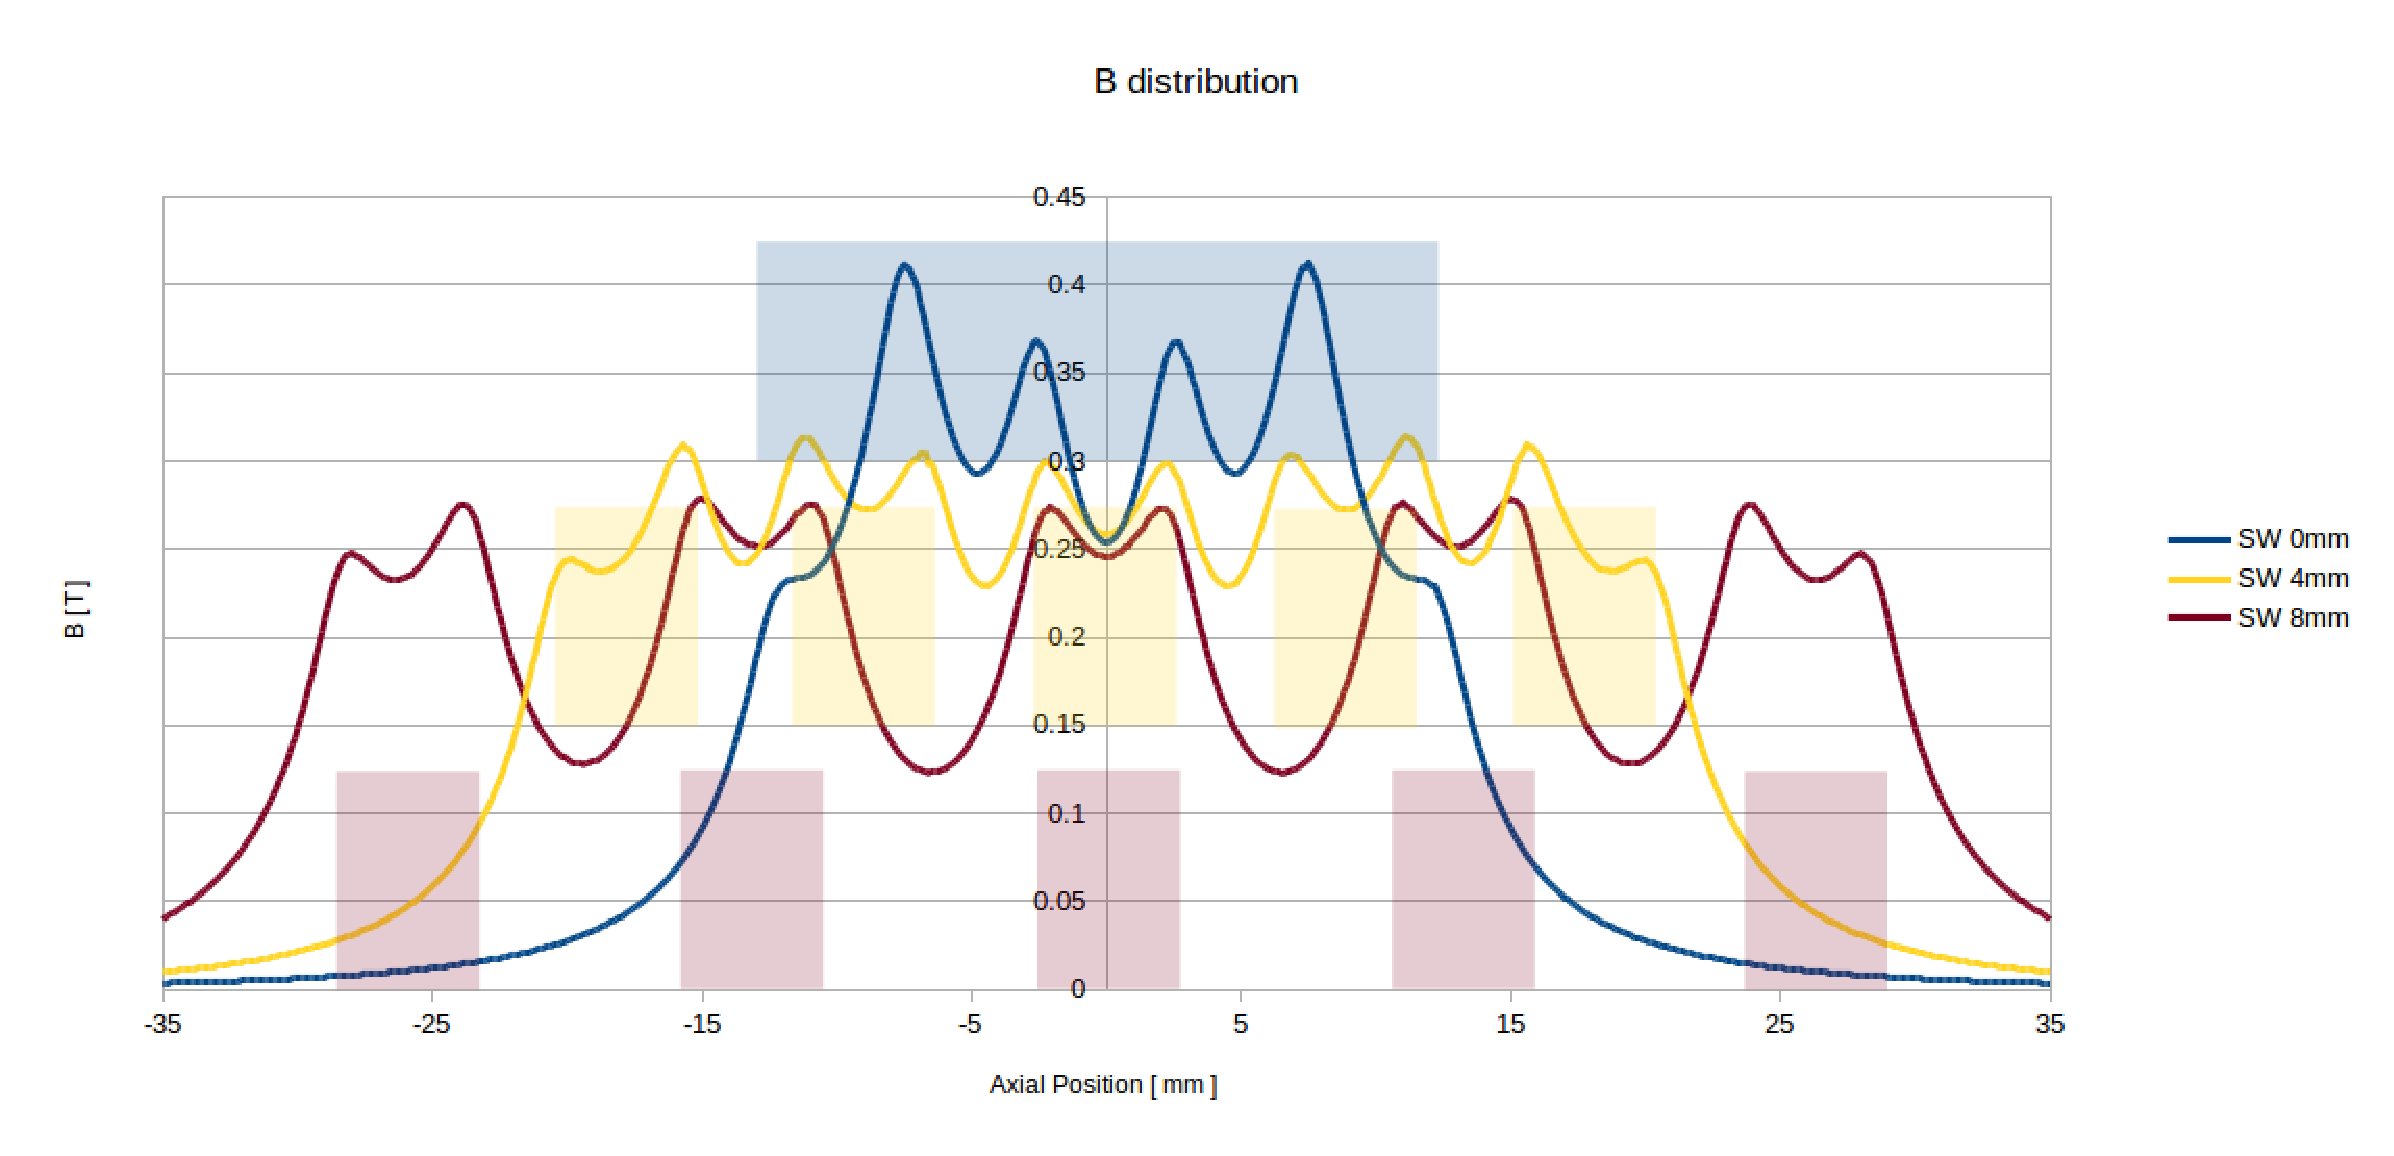
\includegraphics[width=125mm]{B_sw.eps}
    \end{center}
    \caption{磁石の間隔を変化させた際の磁束密度の大きさの分布}
    \label{fig:B_sw}
  \end{figure}

\newpage 

  \section{おわりに}
本研究では磁気解析システムの構築及び分析を行った. 
加工面各点における磁束密度および磁束密度の径方向への勾配に関する評価を行った結果, いずれも1対1に単純に加工原理を説明できないことが分かった. よって本研究の成果をもとに, 軸方向の磁束密度分布や, 面的な磁束密度分布, さらにこれらの複合的な関係を評価し, 実験的加工量との対応を調査することが不可欠であると考えられる. 


  \section*{謝辞}
まず, 本研究に関してご指導いただいた所属研究室の西田先生, 櫻井先生, 池田先生にこの場を借りて感謝の意を表したいと思います. 特に直接的にご指導いただいた池田先生には, 様々な面で大変お世話になりました. 深く御礼申し上げます. また実験データの提供および様々なアドバイスと試料の作成をおこなってくれた西田研究室の学生の協力なくして本研究は行うことができませんでした. そして本研究への協力を惜しまず実質的な共同研究者であった塚田君への感謝の意を示します. 

  \begin{thebibliography}{99}

%参考文献


    \bibitem{磁性流体}
 山口博司 ( 2011 ) .  磁性流体, 森北出版.

    \bibitem{精密機械加工の原理}
 安永暢男 , 高木純一郎 . 精密機械加工の原理 工業調査会 

    \bibitem{機能性流体}
 島田邦雄 ( 2008 ) .  機能性流体力学(12),機械の研究,Vol.60,No.9,pp.974-978 .

    \bibitem{西田}
 Hitoshi Nishida, Kunio Shimada, Ichro Yoshino ( 2012 ). Study of Micro Processing for Inner Tube Walls Utilizing Magnetic Compound Fluid {\it Journal of Japanese Society for Experimental mechanics}, vol 12, No 4, pp.361-368 .   

    \bibitem{塚田}
 塚田, 池田, 平松, 櫻井, 西田. 磁気機能性流体を用いた円管内面マイクロ加工のための磁界解析 第38回 日本応用磁気学会学術講演会 講演番号: 2aF-2 (2014).

    \bibitem{MCF磁気特性}
 Kunio Shimada , Hideo Oka ( 2005 ) . Magnetc characteristics of magnetic compound fluid ( MCF ) under DC and AC magnetic fields { \it Journal of Magnetic Materials}, 290 - 291 , 804 - 807 .

    \bibitem{楠}
 楠裕也 ( 2013 ).  磁気機能性流体を用いた垂直円管内面加工の基本特性, 富山高等専門学校(本郷キャンパス)専攻科特別研究論文集, 平成25年度, pp.9-14. 

    \bibitem{KMmacro}
 ベーカー街の物置/KMmacro, www.geocities.jp/trick\_room/kmmacro.html\#26 .

    \bibitem{RR}
 The R project for statistical computing, www.r-project.org .

\begin{comment}
    \bibitem{Huiru}
 Huiru Guo , Yongbo Wu , Dong Lu , Masakazu Fujimoto , Mitsuyoshi Nomura ( 2014 ) .  Effect of pressure and shear stress on material removal rate in ultra-fine polishing of optical glass with magnetic compound fluid slurry { \it Journal of Material Processing Technology , 214 , 2759 – 2769 . }

    \bibitem{ICT}
    International Critical Table

\end{comment}

  \end{thebibliography}

\newpage


\end{document}
